\documentclass[12pt,a4paper]{article}
\usepackage{fontspec}
\setmainfont{Times New Roman}
\usepackage{geometry}
\usepackage{graphicx}
\usepackage{booktabs}
\usepackage{float}
\usepackage{longtable}
\usepackage{hyperref}
\usepackage{caption}
\usepackage{array}
\geometry{margin=1in}

\title{Dự báo chuỗi thời gian bán lẻ có xét đến tình trạng hết hàng trên FreshRetailNet-50K}
\author{}
\date{}

\begin{document}
\maketitle

\begin{abstract}
Báo cáo này trình bày một quy trình two-stage cho bộ dữ liệu FreshRetailNet-50K: khôi phục latent demand trong các giờ stockout, sau đó dự báo nhu cầu trên recovered demand.
Thí nghiệm sử dụng mẫu 0.1 ở cấp \texttt{series\_id}, giữ nguyên toàn bộ dòng thời gian của các chuỗi được chọn.
Dữ liệu theo ngày được bung thành dữ liệu theo giờ bằng \texttt{hours\_sale} và \texttt{hours\_stock\_status}, rồi aggregate lại thành daily recovered demand cho bài toán dự báo tổng nhu cầu 7 ngày.
Tập dữ liệu cuối cùng có 11640000 quan sát theo giờ và 5000 chuỗi, từ 2024-03-28 00:00:00 đến 2024-07-02 23:00:00.
\end{abstract}

\section{Câu hỏi nghiên cứu và động lực}
Bài toán đặt ra là dự báo lượng bán trong tương lai cho nhiều chuỗi cửa hàng--sản phẩm, đồng thời xét đến tình trạng hết hàng.
Trong bán lẻ, doanh số quan sát được trong lúc hết hàng thường bị kiểm duyệt: bán thấp không nhất thiết là nhu cầu thấp, mà có thể do không còn hàng để bán.
Vì vậy, mô hình cần tận dụng thông tin mùa vụ, lịch, khuyến mãi, thời tiết và đặc biệt là đặc trưng stockout-aware.

\section{Dữ liệu và tiền xử lý}
Dữ liệu gốc gồm \texttt{train.parquet} và \texttt{eval.parquet}.
Sau khi chuẩn hóa, biến \texttt{series\_id} được tạo từ \texttt{city\_id}, \texttt{store\_id} và \texttt{product\_id}.
Các chuỗi bán theo giờ trong \texttt{hours\_sale} được bung thành từng quan sát giờ; trạng thái hết hàng theo giờ được lấy từ \texttt{hours\_stock\_status}.

\begin{table}[H]
\centering
\caption{Tóm tắt chất lượng dữ liệu}
\begin{tabular}{ll}
\toprule
Metric & Value \\
\midrule
Sample fraction & 0.1 \\
Number of rows & 11640000 \\
Number of series & 5000 \\
Number of stores & 866 \\
Number of products & 516 \\
Number of cities & 18 \\
Start date & 2024-03-28 00:00:00 \\
End date & 2024-07-02 23:00:00 \\
Frequency & Hourly rows expanded from hours\_sale and hours\_stock\_status \\
Missing dt count & 0 \\
Duplicate rows & 0 \\
Missing sale\_amount & 0 \\
Stockout rate & 0.24667061855670103 \\
Average sale\_amount & 0.04194150120019913 \\
Median sale\_amount & 0.0 \\
\bottomrule
\end{tabular}
\end{table}

\section{Phân tích khám phá dữ liệu}
Các biểu đồ EDA cho thấy dữ liệu có tính mùa vụ theo giờ, tính thưa cao, và tỷ lệ hết hàng biến động rõ theo thời gian.


\begin{figure}[H]
    \centering
    
\includegraphics[width=0.92\linewidth]{../figures/aggregate_sales_over_time.png}
    \caption{Tổng lượng bán theo giờ theo thời gian.}
    \label{fig:vi-aggregate-sales}
\end{figure}


\begin{figure}[H]
    \centering
    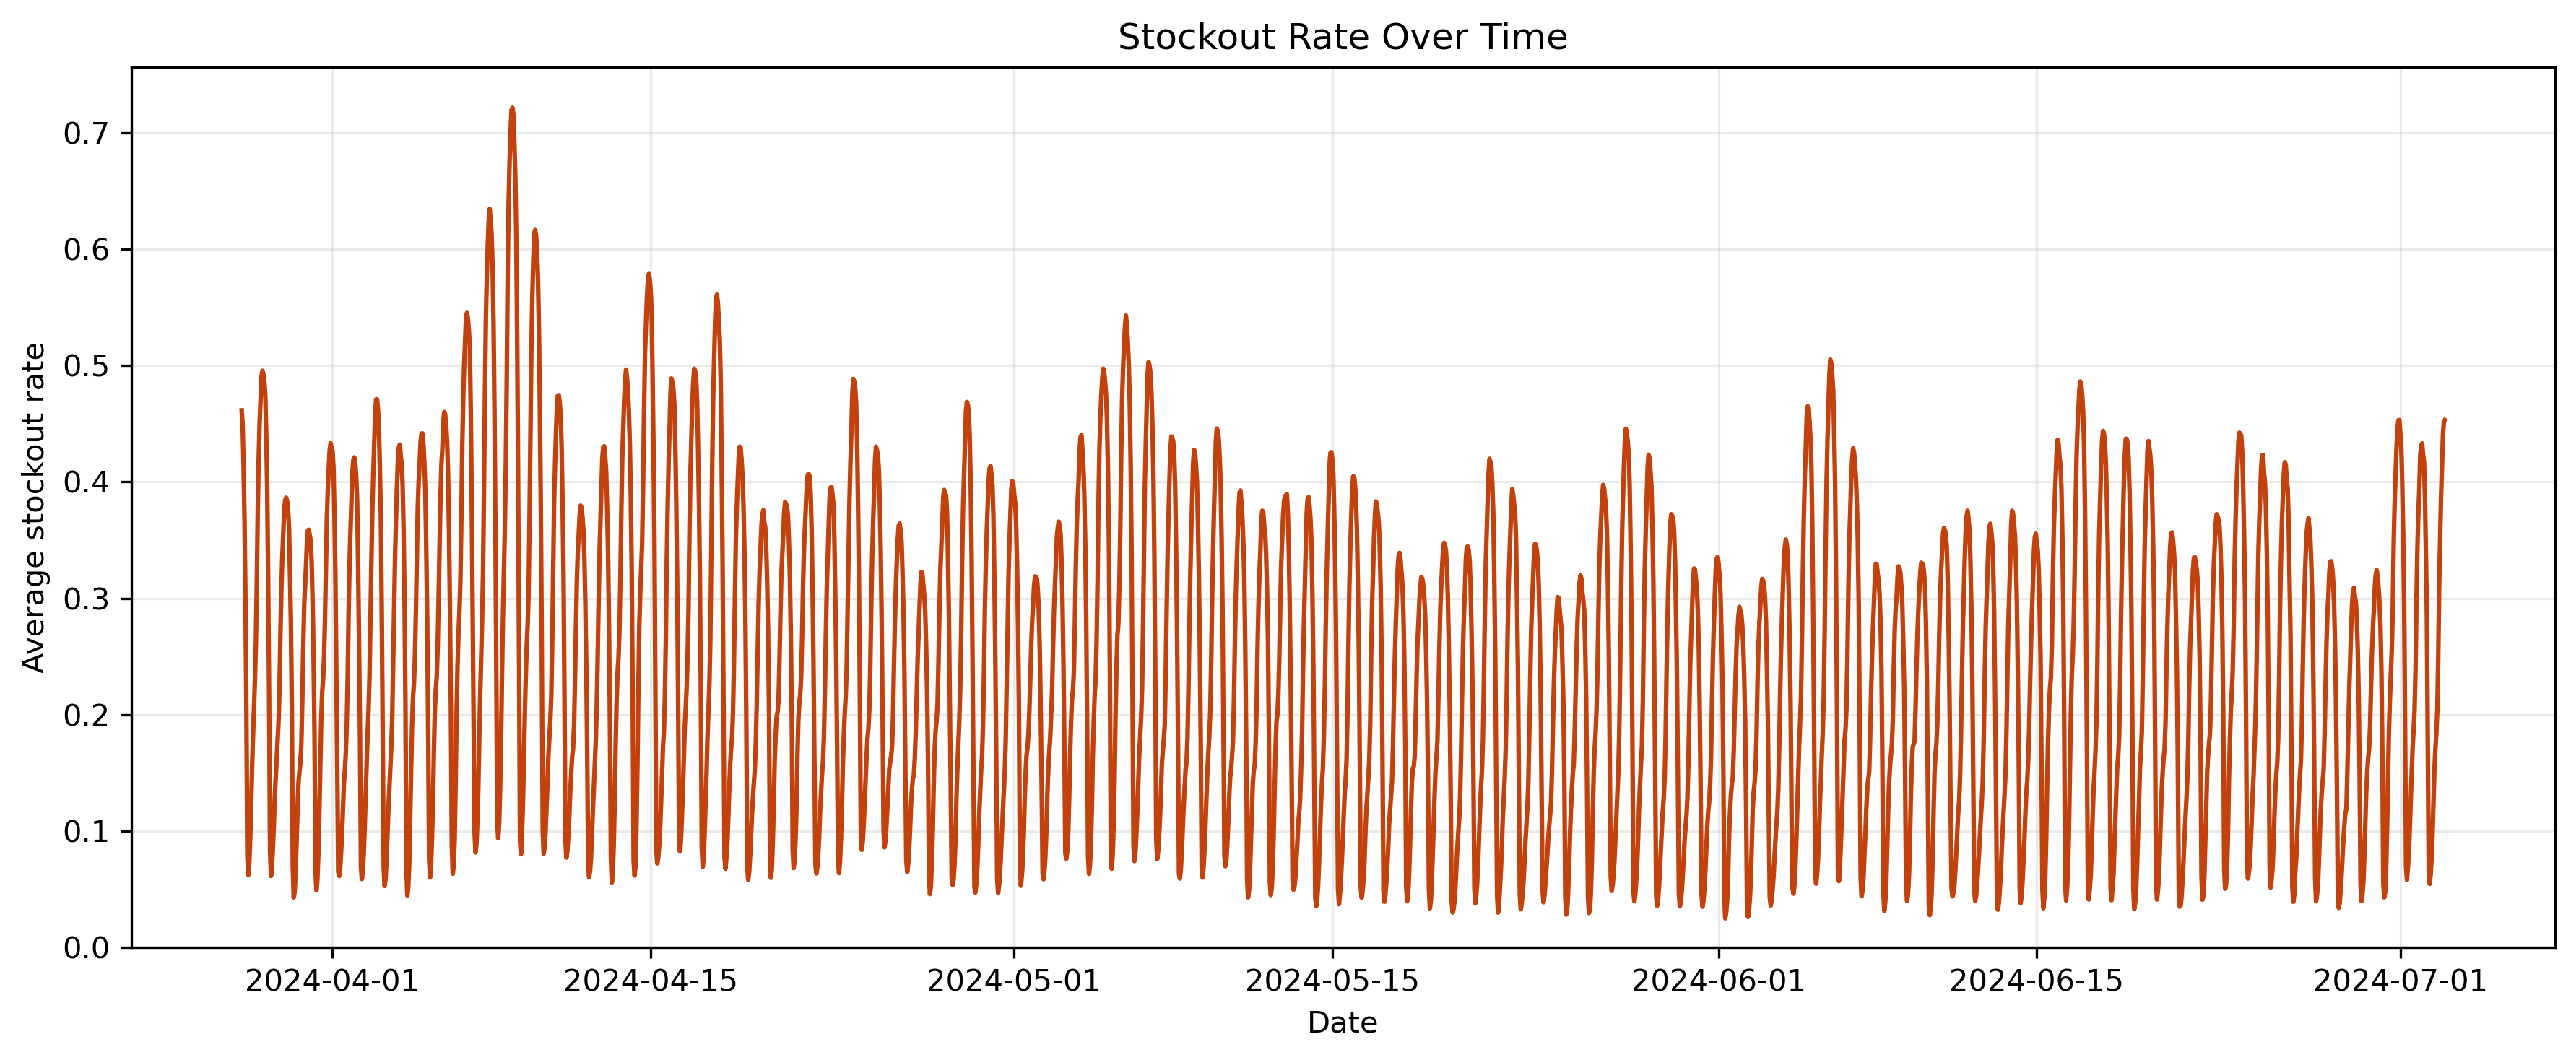
\includegraphics[width=0.92\linewidth]{../figures/stockout_rate_over_time.png}
    \caption{Tỷ lệ hết hàng theo giờ theo thời gian.}
    \label{fig:vi-stockout-rate}
\end{figure}


\begin{figure}[H]
    \centering
    
\includegraphics[width=0.78\linewidth]{../figures/sale_amount_distribution.png}
    \caption{Phân phối lượng bán theo giờ.}
    \label{fig:vi-sale-dist}
\end{figure}


\begin{figure}[H]
    \centering
    
\includegraphics[width=0.78\linewidth]{../figures/log_sale_amount_distribution.png}
    \caption{Phân phối log1p của lượng bán theo giờ.}
    \label{fig:vi-log-sale-dist}
\end{figure}


\begin{figure}[H]
    \centering
    
\includegraphics[width=0.78\linewidth]{../figures/sales_by_hour_of_day.png}
    \caption{Lượng bán trung bình theo giờ trong ngày.}
    \label{fig:vi-hour-seasonality}
\end{figure}


\begin{figure}[H]
    \centering
    
\includegraphics[width=0.78\linewidth]{../figures/sales_by_day_of_week.png}
    \caption{Lượng bán trung bình theo thứ trong tuần.}
    \label{fig:vi-dow-seasonality}
\end{figure}


\begin{table}[H]
\centering
\caption{Các chuỗi đại diện được chọn để minh họa}
\begin{tabular}{lllll}
\toprule
series\_id & type & total\_sales & stockout\_rate & n\_obs \\
\midrule
4\_11\_267 & high\_volume & 1,896 & 0.6070 & 2328 \\
3\_793\_550 & intermittent & 49.7000 & 0.1907 & 2328 \\
5\_6\_757 & stockout\_heavy & 48.4000 & 0.7371 & 2328 \\
\bottomrule
\end{tabular}
\end{table}


\begin{figure}[H]
    \centering
    
\includegraphics[width=0.92\linewidth]{../figures/representative_series_high_volume.png}
    \caption{Chuỗi đại diện có tổng lượng bán cao.}
    \label{fig:vi-rep-high}
\end{figure}


\begin{figure}[H]
    \centering
    
\includegraphics[width=0.92\linewidth]{../figures/representative_series_intermittent.png}
    \caption{Chuỗi đại diện có nhu cầu thưa/ngắt quãng.}
    \label{fig:vi-rep-intermittent}
\end{figure}


\begin{figure}[H]
    \centering
    
\includegraphics[width=0.92\linewidth]{../figures/representative_series_stockout_heavy.png}
    \caption{Chuỗi đại diện có tỷ lệ hết hàng cao.}
    \label{fig:vi-rep-stockout}
\end{figure}


\section{Tính dừng, ACF/PACF và nhận dạng mô hình}
ADF và KPSS được dùng để kiểm tra tính dừng trên chuỗi tổng hợp và các chuỗi đại diện.
Kết quả cho thấy sai phân bậc một và sai phân mùa vụ lag 24 giúp cải thiện tính dừng, phù hợp với việc sử dụng các đặc trưng lag 24 giờ và lag 168 giờ.

\begin{table}[H]
\centering
\caption{Kết quả kiểm định ADF/KPSS}
\resizebox{\linewidth}{!}{%
\begin{tabular}{llllll}
\toprule
Series & Transformation & ADF p-value & KPSS p-value & Conclusion & N \\
\midrule
aggregate\_hourly\_sales & original & 0.0000 & 0.0100 & mixed evidence & 2328 \\
aggregate\_hourly\_sales & log1p & 0.0000 & 0.0100 & mixed evidence & 2328 \\
aggregate\_hourly\_sales & first\_difference & 0.0000 & 0.1000 & stationary & 2327 \\
aggregate\_hourly\_sales & seasonal\_difference\_lag\_24 & 0.0000 & 0.1000 & stationary & 2304 \\
high\_volume\_series & original & 0.3070 & 0.0100 & non-stationary & 2328 \\
high\_volume\_series & log1p & 0.4265 & 0.0100 & non-stationary & 2328 \\
high\_volume\_series & first\_difference & 0.0000 & 0.1000 & stationary & 2327 \\
high\_volume\_series & seasonal\_difference\_lag\_24 & 0.0000 & 0.1000 & stationary & 2304 \\
intermittent\_series & original & 0.0000 & 0.1000 & stationary & 2328 \\
intermittent\_series & log1p & 0.0000 & 0.1000 & stationary & 2328 \\
intermittent\_series & first\_difference & 0.0000 & 0.1000 & stationary & 2327 \\
intermittent\_series & seasonal\_difference\_lag\_24 & 0.0000 & 0.1000 & stationary & 2304 \\
stockout\_heavy\_series & original & 0.0058 & 0.0100 & mixed evidence & 2328 \\
stockout\_heavy\_series & log1p & 0.0031 & 0.0100 & mixed evidence & 2328 \\
stockout\_heavy\_series & first\_difference & 0.0000 & 0.1000 & stationary & 2327 \\
stockout\_heavy\_series & seasonal\_difference\_lag\_24 & 0.0000 & 0.1000 & stationary & 2304 \\
\bottomrule
\end{tabular}
}
\end{table}


\begin{figure}[H]
    \centering
    
\includegraphics[width=0.85\linewidth]{../figures/acf_aggregate_sales.png}
    \caption{ACF của chuỗi tổng hợp theo giờ.}
    \label{fig:vi-acf-aggregate}
\end{figure}


\begin{figure}[H]
    \centering
    
\includegraphics[width=0.85\linewidth]{../figures/pacf_aggregate_sales.png}
    \caption{PACF của chuỗi tổng hợp theo giờ.}
    \label{fig:vi-pacf-aggregate}
\end{figure}


\subsection{Phân tích phổ tần số}
Ngoài ACF/PACF, báo cáo dùng periodogram để kiểm tra seasonality trong miền tần số.
Mục tiêu là xác nhận liệu các chu kỳ được dùng trong feature engineering và baseline có xuất hiện rõ trong dữ liệu hay không.
Với chuỗi hourly aggregate, peak mạnh nhất nằm ở khoảng 24 giờ, ủng hộ việc dùng lag 24 giờ và các đặc trưng theo giờ trong ngày.
Một peak yếu hơn gần 168 giờ cũng xuất hiện, phù hợp với seasonality theo tuần.
Sau khi chuyển sang daily recovered demand, peak lớn nhất nằm gần 7 ngày, củng cố lựa chọn lag 7/14/28 ngày và seasonal naive theo tuần cho bài toán two-stage.


\begin{figure}[H]
    \centering
    
\includegraphics[width=0.88\linewidth]{../figures/spectrum_hourly_aggregate_sales.png}
    \caption{Phổ tần số của aggregate observed sales theo giờ.}
    \label{fig:vi-spectrum-hourly}
\end{figure}


\begin{table}[H]
\centering
\caption{Các peak chu kỳ lớn nhất của hourly aggregate sales}
\begin{tabular}{lllll}
\toprule
Rank & Period & Frequency & Power & Period unit \\
\midrule
1 & 24.0000 & 0.0417 & 0.6365 & hours \\
2 & 8.0000 & 0.1250 & 0.1182 & hours \\
3 & 12.0000 & 0.0833 & 0.0559 & hours \\
4 & 6.0000 & 0.1667 & 0.0325 & hours \\
5 & 164.5714 & 0.0061 & 0.0106 & hours \\
6 & 28.0976 & 0.0356 & 0.0099 & hours \\
7 & 12.9438 & 0.0773 & 0.0058 & hours \\
8 & 20.9455 & 0.0477 & 0.0053 & hours \\
\bottomrule
\end{tabular}
\end{table}


\begin{figure}[H]
    \centering
    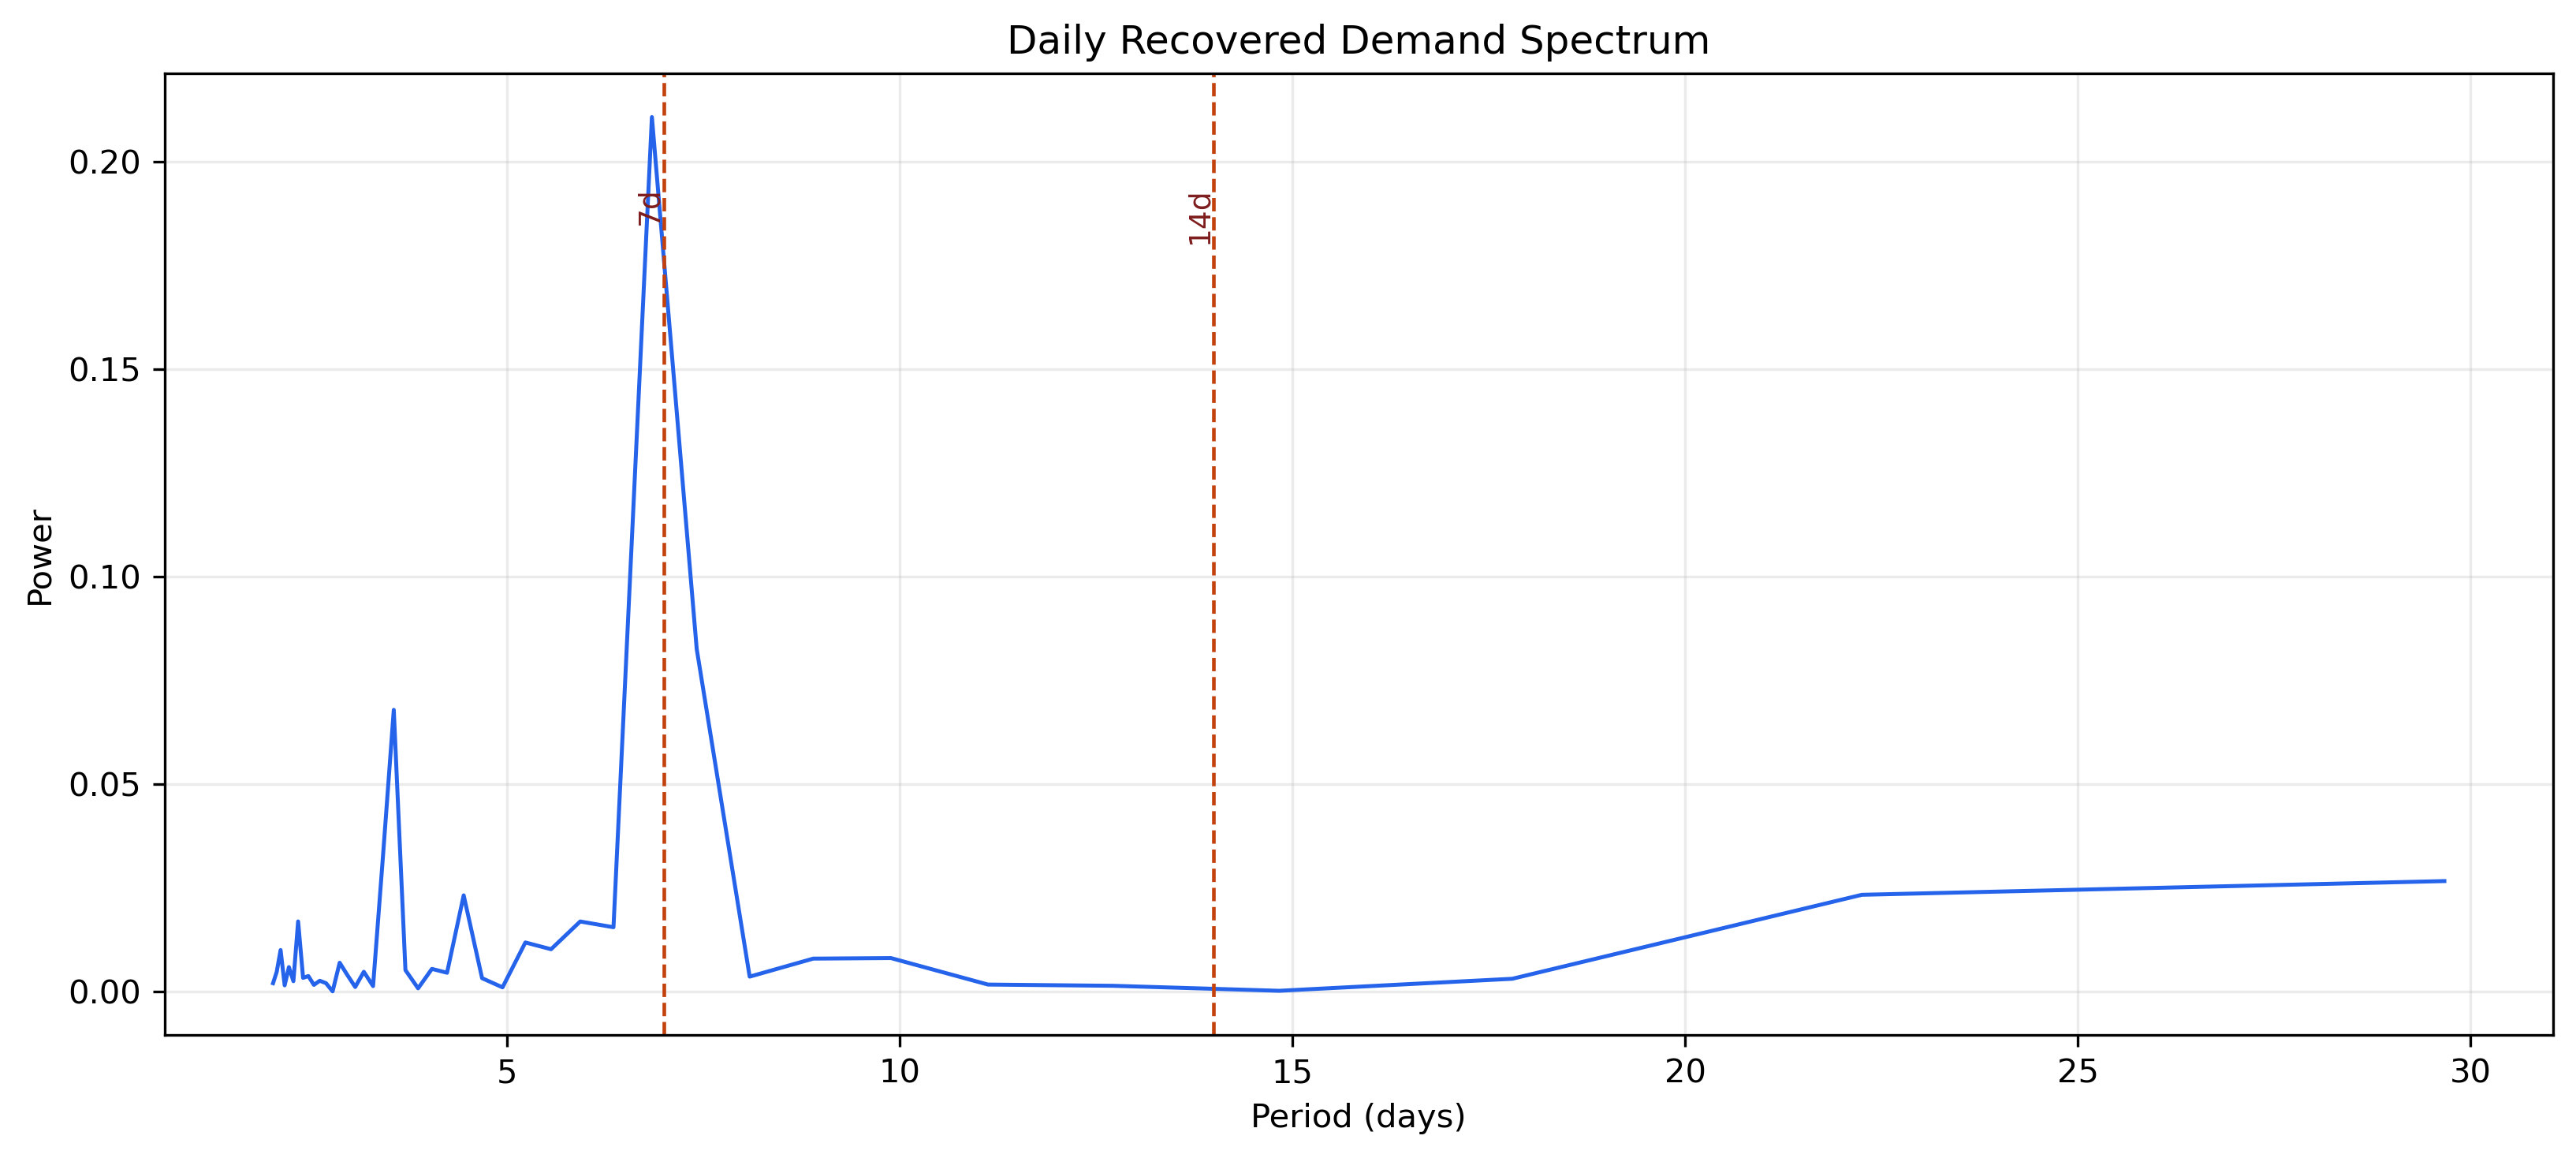
\includegraphics[width=0.88\linewidth]{../figures/spectrum_daily_recovered_demand.png}
    \caption{Phổ tần số của daily recovered demand.}
    \label{fig:vi-spectrum-daily}
\end{figure}


\begin{table}[H]
\centering
\caption{Các peak chu kỳ lớn nhất của daily recovered demand}
\begin{tabular}{lllll}
\toprule
Rank & Period & Frequency & Power & Period unit \\
\midrule
1 & 6.8462 & 0.1461 & 0.2108 & days \\
2 & 3.5600 & 0.2809 & 0.0679 & days \\
3 & 4.4500 & 0.2247 & 0.0232 & days \\
4 & 2.3421 & 0.4270 & 0.0169 & days \\
5 & 5.9333 & 0.1685 & 0.0169 & days \\
6 & 5.2353 & 0.1910 & 0.0118 & days \\
7 & 2.1190 & 0.4719 & 0.0100 & days \\
8 & 9.8889 & 0.1011 & 0.0081 & days \\
\bottomrule
\end{tabular}
\end{table}

\section{Thiết kế đặc trưng và chia tập dữ liệu}
Các đặc trưng được tạo gồm calendar features, lag features, rolling features, promotion/weather features và stockout-aware features.
Để tránh rò rỉ dữ liệu, tất cả rolling features đều được shift một bước trước khi tính rolling.
Mục tiêu dự báo là \texttt{target\_h1} và \texttt{target\_h24}, tương ứng với dự báo trước 1 giờ và 24 giờ.

\begin{table}[H]
\centering
\caption{Chia train/validation/test theo thời gian}
\begin{tabular}{lllll}
\toprule
Split & Start date & End date & Rows & Series \\
\midrule
Train & 2024-03-28 & 2024-06-10 23:00:00 & 9000000 & 5000 \\
Validation & 2024-06-11 & 2024-06-17 23:00:00 & 840000 & 5000 \\
Test & 2024-06-18 & 2024-07-01 23:00:00 & 1680000 & 5000 \\
\bottomrule
\end{tabular}
\end{table}

Với pipeline two-stage, phần forecasting cuối cùng được định nghĩa ở cấp ngày theo \textbf{forecast origin}.
Mỗi dòng dự báo tại ngày $t$ có target là tổng recovered demand trong 7 ngày sau đó, tức từ $t+1$ đến $t+7$.
Vì vậy, báo cáo lưu thêm bảng split riêng cho daily forecasting để phân biệt rõ origin window và target window.

\begin{table}[H]
\centering
\caption{Chia tập cho daily 7-day forecasting theo forecast origin}
\resizebox{\linewidth}{!}{%
\begin{tabular}{lllllll}
\toprule
Split & Origin start & Origin end & Target window start & Target window end & Rows & Series \\
\midrule
Train & 2024-03-28 & 2024-06-03 & 2024-03-29 & 2024-06-10 & 340000 & 5000 \\
Validation & 2024-06-04 & 2024-06-10 & 2024-06-05 & 2024-06-17 & 35000 & 5000 \\
Test & 2024-06-11 & 2024-06-24 & 2024-06-12 & 2024-07-01 & 70000 & 5000 \\
\bottomrule
\end{tabular}
}
\end{table}

\section{Lý do lựa chọn mô hình}
Mô hình chính được chọn là LightGBM vì bài toán có nhiều chuỗi store--product, dữ liệu thưa, nhiều biến ngoại sinh và nhiều đặc trưng phi tuyến.
Huấn luyện một mô hình ARIMA/SARIMA riêng cho từng chuỗi sẽ khó mở rộng, không ổn định với chuỗi thưa và khó đưa đầy đủ thông tin khuyến mãi, thời tiết, stockout.
Ridge được giữ lại như baseline tuyến tính dễ diễn giải.
SARIMAX được dùng trên chuỗi tổng hợp như một đối chứng cổ điển, nhưng không thay thế cho mô hình toàn cục ở cấp sản phẩm--cửa hàng.
Deep learning không được chọn làm mô hình chính vì yêu cầu nhiều tài nguyên và tuning hơn, trong khi LightGBM cho tỉ lệ hiệu quả/độ phức tạp tốt hơn trong bối cảnh đồ án tái lập được.

\section{Tiếp cận theo hướng của paper/repository}
Paper FreshRetailNet-50K và repository baseline không xem đây chỉ là bài toán dự báo doanh số quan sát được.
Hướng tiếp cận chính là two-stage censored demand modeling:
\begin{enumerate}
    \item Khôi phục latent demand trong các giờ stockout vì observed sales bị kiểm duyệt.
    \item Dùng recovered demand để huấn luyện mô hình dự báo nhu cầu robust hơn.
\end{enumerate}

Trong đồ án này, ta triển khai một phiên bản nhẹ và tái lập được của ý tưởng đó.
Để tránh leakage theo thời gian, phần recovery trong train period dùng expanding window theo block tuần: mỗi block chỉ được recover bằng mô hình học từ các giờ không stockout trong quá khứ.
Validation và test được recover bằng final recovery model train trên các giờ không stockout thuộc train period.
Với các giờ stockout, mô hình tạo \texttt{imputed\_demand\_raw}, sau đó hiệu chỉnh bằng calibration factor học từ validation non-stockout rows.
Phần lost demand được tính bằng \texttt{max(calibrated imputed demand - observed sales, 0)} và được cap tại phân vị q90 của lost demand dương để tránh một số giờ stockout làm tổng demand tăng quá mức.
Cuối cùng, \texttt{recovered\_demand = observed sales + capped lost demand}.
Sau đó recovered demand theo giờ được aggregate thành daily demand để làm bài toán dự báo tổng nhu cầu 7 ngày tiếp theo.

\subsection{Cơ chế expanding-window recovery}
Quy trình recovery được thiết kế theo nguyên tắc point-in-time: tại một thời điểm bất kỳ, mô hình không được sử dụng dữ liệu ở tương lai để khôi phục demand ở hiện tại.
Sơ đồ dưới đây tóm tắt toàn bộ luồng xử lý từ dữ liệu gốc đến latent demand recovery và forecasting.


\begin{figure}[H]
    \centering
    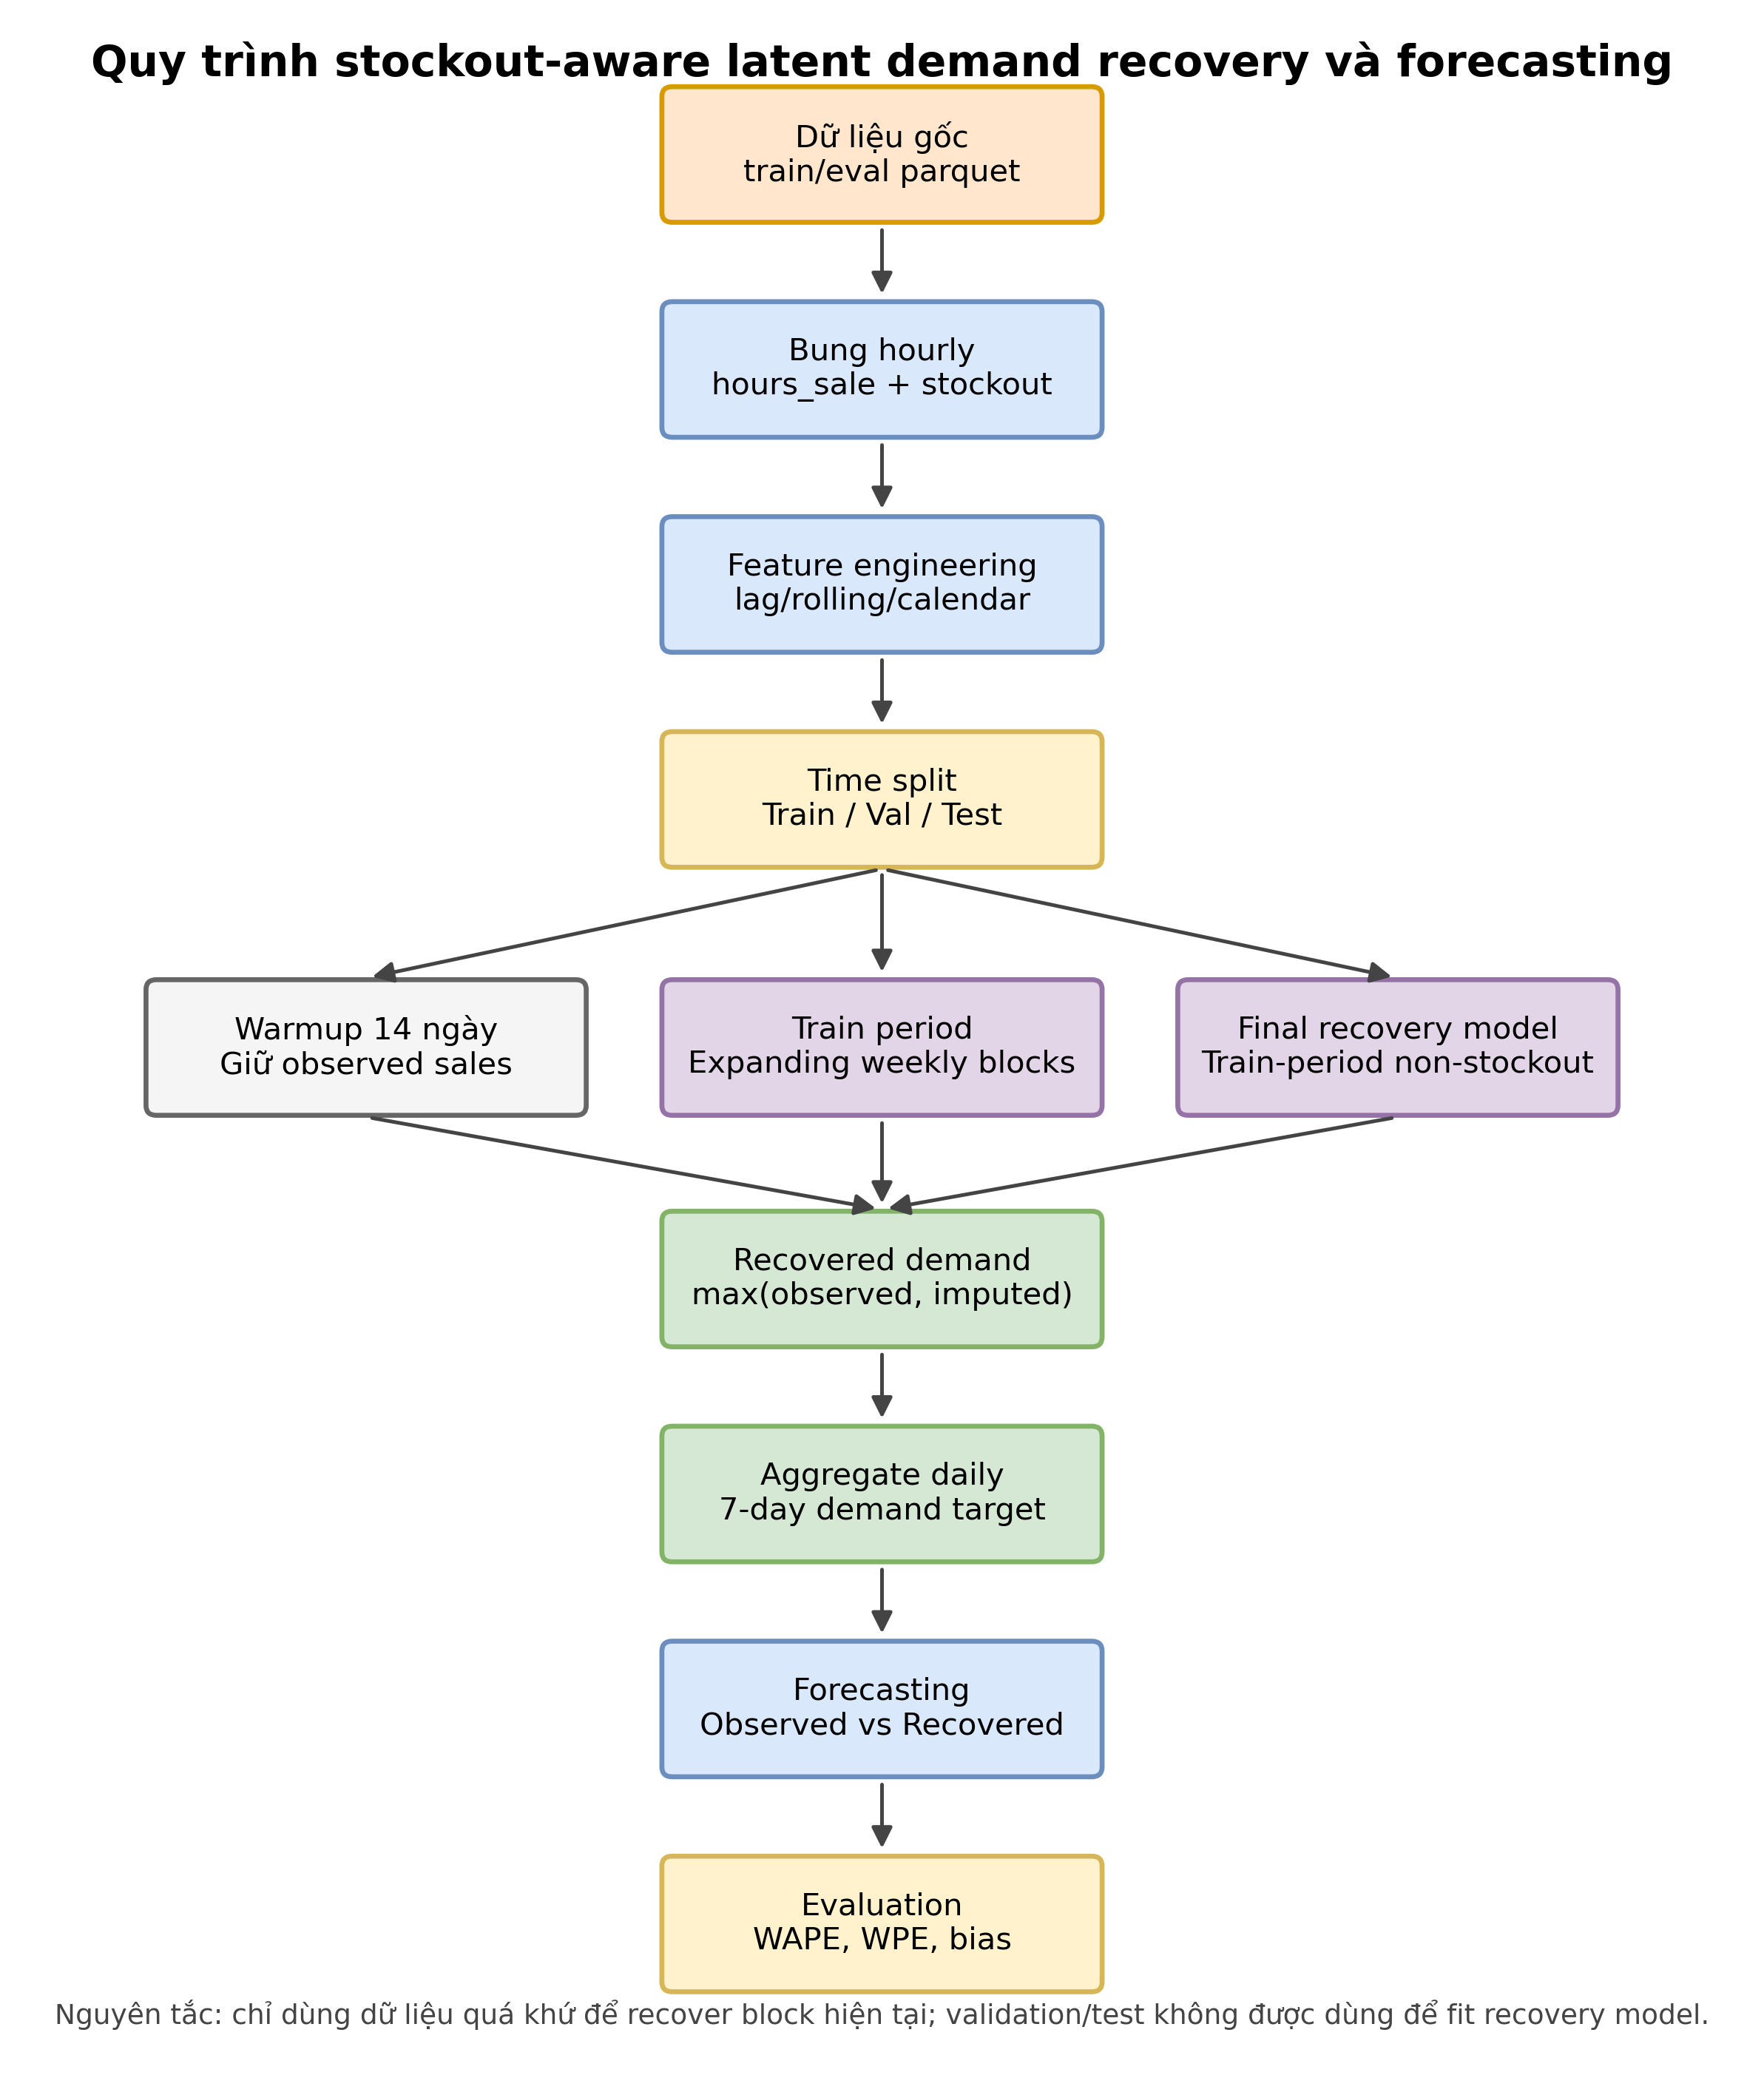
\includegraphics[width=0.88\linewidth]{../figures/owner_expanding_window_process.png}
    \caption{Sơ đồ quy trình expanding-window latent demand recovery và forecasting.}
    \label{fig:vi-expanding-window-process}
\end{figure}


\subsubsection{Quy trình xử lý riêng cho expanding-window recovery}
Phần recovery được tách thành một quy trình riêng vì đây là bước dễ gây leakage nhất trong bài toán latent demand.
Ý tưởng cốt lõi là mô phỏng đúng bối cảnh triển khai thực tế: khi cần khôi phục nhu cầu ở tuần hiện tại, mô hình chỉ được biết các quan sát không stockout đã xảy ra trước tuần đó.
Do đó, ngay cả trong train period, ta không dùng dữ liệu của các ngày phía sau để recover các ngày phía trước.


\begin{figure}[H]
    \centering
    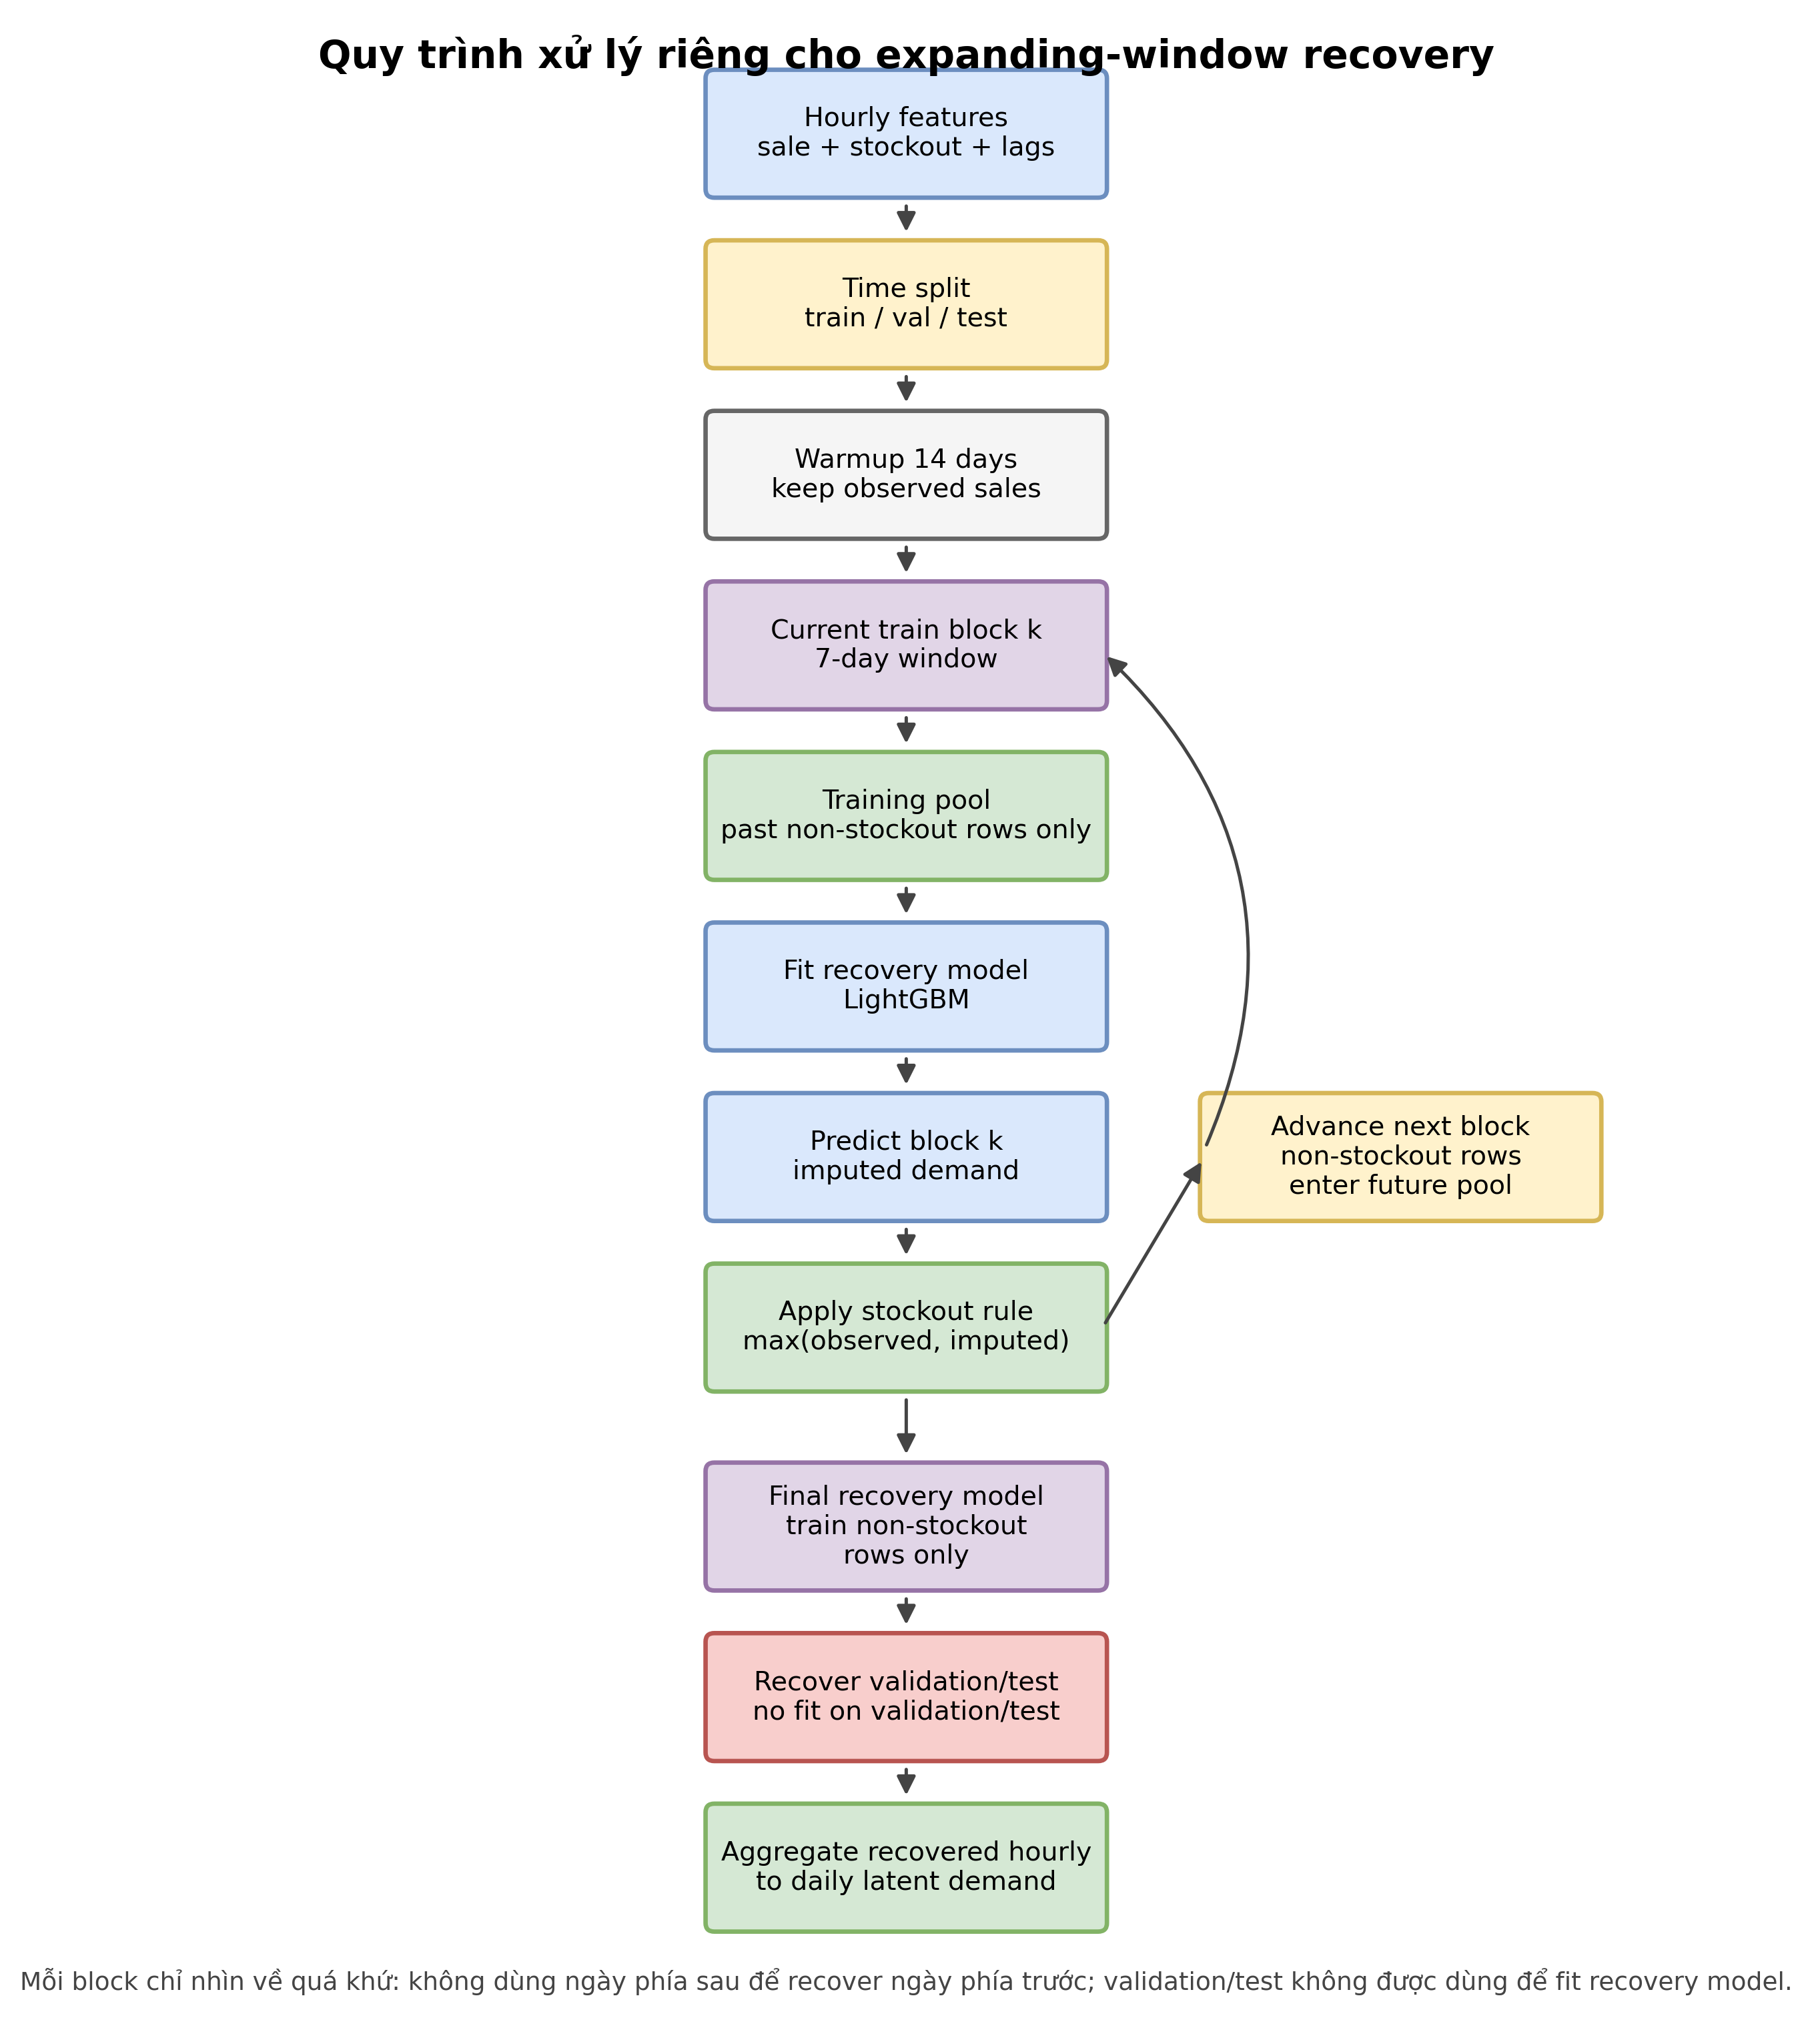
\includegraphics[width=0.9\linewidth]{../figures/owner_expanding_window_recovery_detail.png}
    \caption{Quy trình xử lý riêng cho expanding-window latent demand recovery.}
    \label{fig:vi-expanding-window-recovery-detail}
\end{figure}


Quy trình chi tiết gồm các bước:
\begin{enumerate}
    \item \textbf{Sắp xếp dữ liệu theo thời gian}: toàn bộ hourly frame được sort theo \texttt{dt}, sau đó chia train/validation/test theo mốc thời gian cố định.
    \item \textbf{Giữ warmup 14 ngày đầu}: giai đoạn này chưa đủ lịch sử để fit recovery model ổn định nên \texttt{recovered\_demand} được đặt bằng observed sales.
    \item \textbf{Tạo block recovery trong train period}: phần train sau warmup được chia thành các block 7 ngày liên tiếp.
    \item \textbf{Fit model theo nguyên tắc quá khứ}: với block thứ $k$, tập train của recovery model chỉ gồm các dòng có \texttt{dt < block\_start} và \texttt{stockout\_flag = 0}.
    \item \textbf{Recover block hiện tại}: model dự đoán \texttt{imputed\_demand} cho block $k$; với dòng stockout, ta chỉ cộng thêm phần lost demand dương sau calibration và cap, nên nhu cầu recovered không thấp hơn doanh số đã bán thật nhưng cũng không bị phóng đại bởi các dự đoán cực trị.
    \item \textbf{Di chuyển cửa sổ}: sau khi xử lý xong block $k$, block này trở thành quá khứ cho block $k+1$, nhưng chỉ các dòng \texttt{non-stockout} mới được dùng để fit các model sau.
\end{enumerate}
Sau khi train period kết thúc, một final recovery model được fit trên toàn bộ non-stockout rows của train period và chỉ dùng để recover validation/test.
Cách này giữ đúng point-in-time constraint: validation/test không tham gia fit model, và mỗi block trong train cũng không nhìn thấy tương lai của chính nó.

Mốc warmup 14 ngày được chọn như một thỏa hiệp giữa độ ổn định của recovery model và lượng dữ liệu còn lại để recover.
Vì dữ liệu có mùa vụ theo giờ và theo tuần, 14 ngày tương ứng hai chu kỳ tuần đầy đủ, giúp mô hình nhìn thấy ít nhất hai lần lặp của các pattern theo thứ trong tuần và cuối tuần.
Khoảng này cũng đủ để các đặc trưng lag/rolling ngắn hạn như lag 24 giờ, lag 168 giờ, rolling 24 giờ và rolling 168 giờ bắt đầu có ý nghĩa hơn trước khi fit recovery model đầu tiên.
Nếu warmup quá ngắn, model recovery đầu tiên dễ học từ lịch sử quá ít và impute stockout thiếu ổn định; nếu quá dài, nhiều giờ stockout đầu kỳ bị giữ nguyên observed sales, làm giảm lợi ích của latent demand recovery.
Do đó, 14 ngày là lựa chọn thực dụng cho đồ án: đủ bao phủ seasonality tuần nhưng không làm mất quá nhiều train period.

Các bước cụ thể như sau:
\begin{enumerate}
    \item \textbf{Warmup period}: 14 ngày đầu được giữ nguyên observed sales vì chưa đủ lịch sử để train recovery model ổn định.
    \item \textbf{Chia train period thành block tuần}: sau warmup, train period được chia thành các block 7 ngày liên tiếp.
    \item \textbf{Train recovery cho từng block}: với mỗi block, LightGBM recovery model chỉ được train trên các dòng \texttt{non-stockout} nằm trước thời điểm bắt đầu block.
    \item \textbf{Recover block hiện tại}: model vừa train được dùng để ước lượng \texttt{imputed\_demand} cho block hiện tại; nếu dòng đó stockout, recovered demand bằng observed sales cộng phần lost demand đã calibration và cap.
    \item \textbf{Validation/Test}: sau khi kết thúc train period, một final recovery model được train trên toàn bộ non-stockout rows của train period và dùng để recover validation/test.
\end{enumerate}
Cách làm này tránh cả hai dạng leakage: không dùng validation/test để fit recovery model, và cũng không dùng các ngày phía sau trong train period để recover các ngày phía trước.

\begin{table}[H]
\centering
\caption{Tóm tắt khôi phục latent demand}
\begin{tabular}{ll}
\toprule
Metric & Value \\
\midrule
Observed sales & 482697.09375 \\
Recovered latent demand & 534270.1875 \\
Recovered lost demand & 51572.875 \\
Recovered lift over observed & 0.10684314370155334 \\
Stockout row rate & 0.24652109375 \\
Recovery method & expanding-window weekly recovery \\
Imputation calibration factor & 1.1297638401922185 \\
Lost demand cap quantile & q90 of calibrated positive lost demand \\
Lost demand cap value & 0.06627678871154785 \\
Warmup days kept observed & 14 \\
Recovery block days & 7 \\
Recovery blocks & 9 \\
Final recovery train rows & 400000 \\
Recovery train source & past non-stockout rows only for train blocks; train-period non-stockout rows for validation/test \\
Final recovery train end & 2024-06-10 23:00:00 \\
Validation start & 2024-06-11 00:00:00 \\
Test start & 2024-06-18 00:00:00 \\
\bottomrule
\end{tabular}
\end{table}

\begin{table}[H]
\centering
\caption{Các block expanding-window dùng trong latent demand recovery}
\resizebox{\linewidth}{!}{%
\begin{tabular}{lllll}
\toprule
Block start & Block end & Training end & Training rows & Predicted rows \\
\midrule
2024-04-11 & 2024-04-18 & 2024-04-10 23:00:00 & 400000 & 840000 \\
2024-04-18 & 2024-04-25 & 2024-04-17 23:00:00 & 400000 & 840000 \\
2024-04-25 & 2024-05-02 & 2024-04-24 23:00:00 & 400000 & 840000 \\
2024-05-02 & 2024-05-09 & 2024-05-01 23:00:00 & 400000 & 840000 \\
2024-05-09 & 2024-05-16 & 2024-05-08 23:00:00 & 400000 & 840000 \\
2024-05-16 & 2024-05-23 & 2024-05-15 23:00:00 & 400000 & 840000 \\
2024-05-23 & 2024-05-30 & 2024-05-22 23:00:00 & 400000 & 840000 \\
2024-05-30 & 2024-06-06 & 2024-05-29 23:00:00 & 400000 & 840000 \\
2024-06-06 & 2024-06-11 & 2024-06-05 23:00:00 & 400000 & 600000 \\
\bottomrule
\end{tabular}
}
\end{table}


\begin{figure}[H]
    \centering
    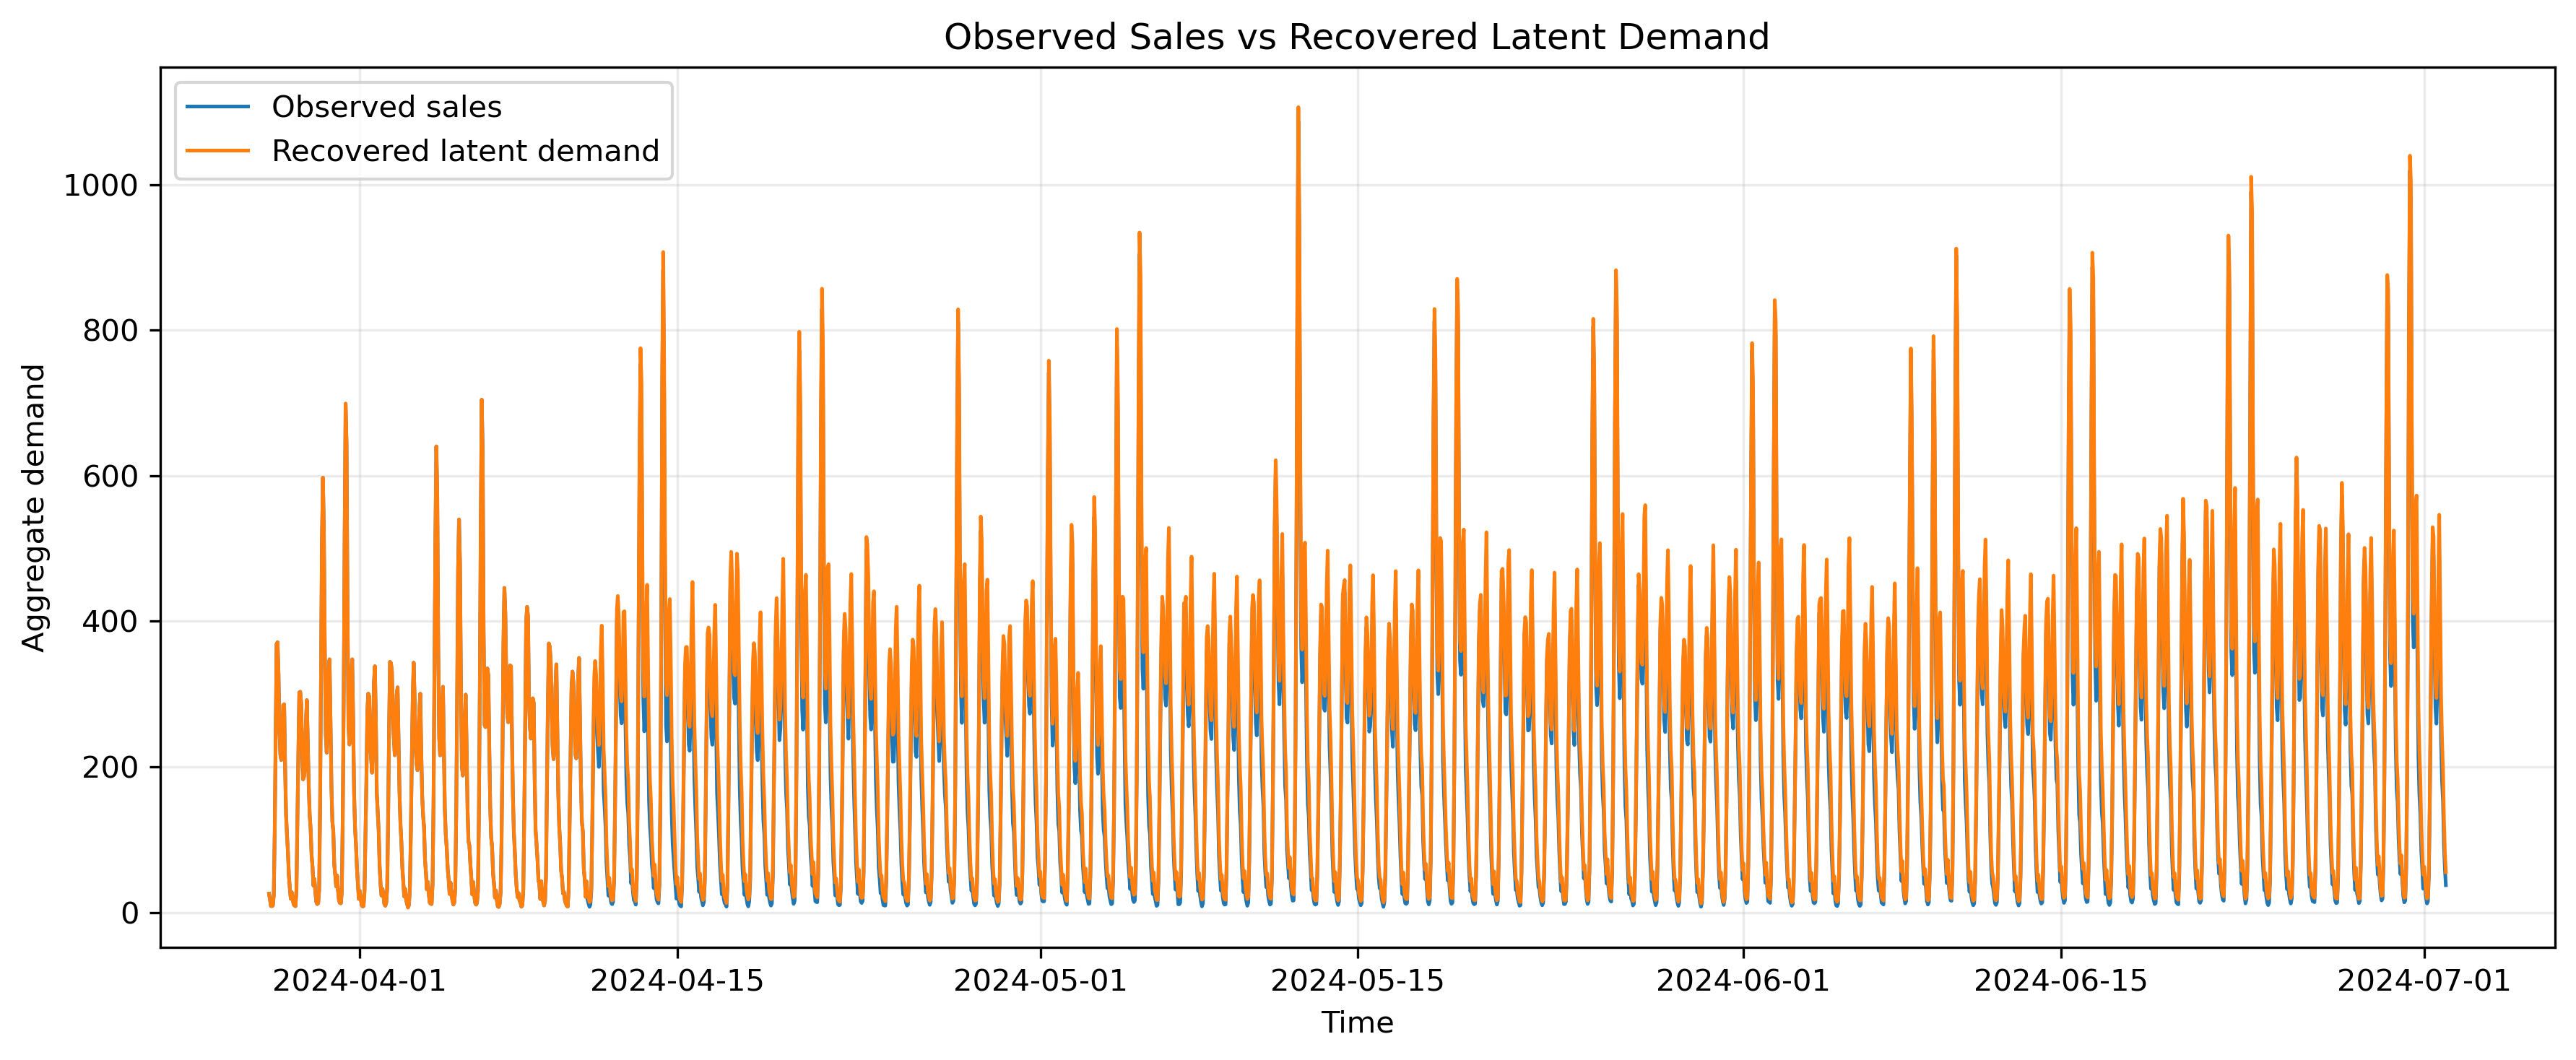
\includegraphics[width=0.92\linewidth]{../figures/owner_observed_vs_recovered_demand.png}
    \caption{Observed sales và recovered latent demand theo thời gian.}
    \label{fig:vi-owner-recovered}
\end{figure}


\subsection{Kiểm tra chất lượng imputation}
Vì recovered demand là biến được ước lượng, báo cáo không xem imputation là ground truth tuyệt đối.
Ta kiểm tra chất lượng impute theo ba hướng.
Thứ nhất, đo tổng mức uplift để xem recovered demand có làm tổng sales tăng quá mức hay không.
Thứ hai, dùng pseudo-stockout validation: lấy các dòng non-stockout trong validation period, giả sử chúng cần impute, rồi so sánh prediction của recovery model với observed sales thật.
Thứ ba, kiểm tra sensitivity khi cap phần recovered lost demand ở các phân vị khác nhau.

\begin{table}[H]
\centering
\caption{Tổng mức uplift do latent-demand imputation}
\begin{tabular}{ll}
\toprule
Metric & Value \\
\midrule
Observed sales & 482,697 \\
Recovered demand & 534,270 \\
Recovered lost demand & 51,573 \\
Recovered lift over observed & 0.1068 \\
Raw calibrated lost demand before cap & 65,368 \\
Cap retained share of raw lost demand & 0.7890 \\
Stockout row share & 0.2465 \\
Recovered lost demand from stockout rows & 51,573 \\
Mean stockout uplift per stockout row & 0.0182 \\
\bottomrule
\end{tabular}
\end{table}

\begin{table}[H]
\centering
\caption{Pseudo-stockout validation trên non-stockout rows}
\begin{tabular}{ll}
\toprule
Metric & Value \\
\midrule
Validation rows & 300000 \\
Pseudo-stockout source & non-stockout rows from validation period \\
RMSE & 0.10030610859394073 \\
MAE & 0.05774029344320297 \\
WAPE & 1.0391554832458496 \\
sMAPE & 1.6277295807119518 \\
Mean prediction / actual ratio & 1.1315665245056152 \\
Mean error actual-minus-imputed & -0.007310444954782724 \\
\bottomrule
\end{tabular}
\end{table}

Do dữ liệu hourly rất thưa và nhiều giá trị nhỏ/zero, row-level WAPE của pseudo-stockout validation có thể nhìn xấu hơn thực tế vận hành.
Vì vậy, báo cáo bổ sung kiểm tra ở cấp aggregate, gồm hourly aggregate, daily aggregate và series-daily aggregate.

\begin{table}[H]
\centering
\caption{Pseudo-stockout validation ở các cấp aggregate}
\resizebox{\linewidth}{!}{%
\begin{tabular}{lllllll}
\toprule
Validation level & RMSE & MAE & WAPE & sMAPE & Prediction / actual ratio & N \\
\midrule
Hourly aggregate & 42.5877 & 21.9068 & 0.2208 & 0.2237 & 1.1316 & 168 \\
Daily aggregate & 450.9920 & 416.6911 & 0.1750 & 0.1677 & 1.1316 & 7 \\
Series daily aggregate & 0.3245 & 0.2155 & 0.4384 & 0.6309 & 1.1316 & 33907 \\
\bottomrule
\end{tabular}
}
\end{table}

Kết quả pseudo-stockout validation cho thấy recovery model có xu hướng dự đoán cao hơn observed sales trên các dòng non-stockout validation.
Vì vậy, phần impute được xem là một proxy có kiểm soát chứ không phải nhãn thật.
Trong pipeline chính, dự đoán raw được chia cho calibration factor 1.1297638401922185 và phần lost demand dương được cap ở giá trị 0.06627678871154785.
Để tránh kết luận phụ thuộc quá mạnh vào impute, báo cáo thêm sensitivity theo mức cap lost demand.

\begin{table}[H]
\centering
\caption{Sensitivity khi cap phần recovered lost demand}
\resizebox{\linewidth}{!}{%
\begin{tabular}{llllll}
\toprule
Scenario & Cap value & Recovered demand & Recovered lost demand & Recovered lift over observed & Share of original recovered lost demand \\
\midrule
Cap lost-demand at q50 & 0.0151 & 505,963 & 23,266 & 0.0482 & 0.3559 \\
Cap lost-demand at q75 & 0.0369 & 523,781 & 41,084 & 0.0851 & 0.6285 \\
Cap lost-demand at q90 & 0.0663 & 534,270 & 51,573 & 0.1068 & 0.7890 \\
Cap lost-demand at q100 & 2.7508 & 548,064 & 65,368 & 0.1354 & 1.0000 \\
\bottomrule
\end{tabular}
}
\end{table}

Ở mức toàn bộ dataset, recovered demand tăng khoảng 10.68\% so với observed sales.
Mức này không làm tổng demand tăng gấp nhiều lần, nhưng một số series có stockout rate rất cao có thể có lift lớn.
Do đó, các series uplift cao được kiểm tra riêng để phát hiện trường hợp forecast phụ thuộc quá mạnh vào imputation.


\begin{figure}[H]
    \centering
    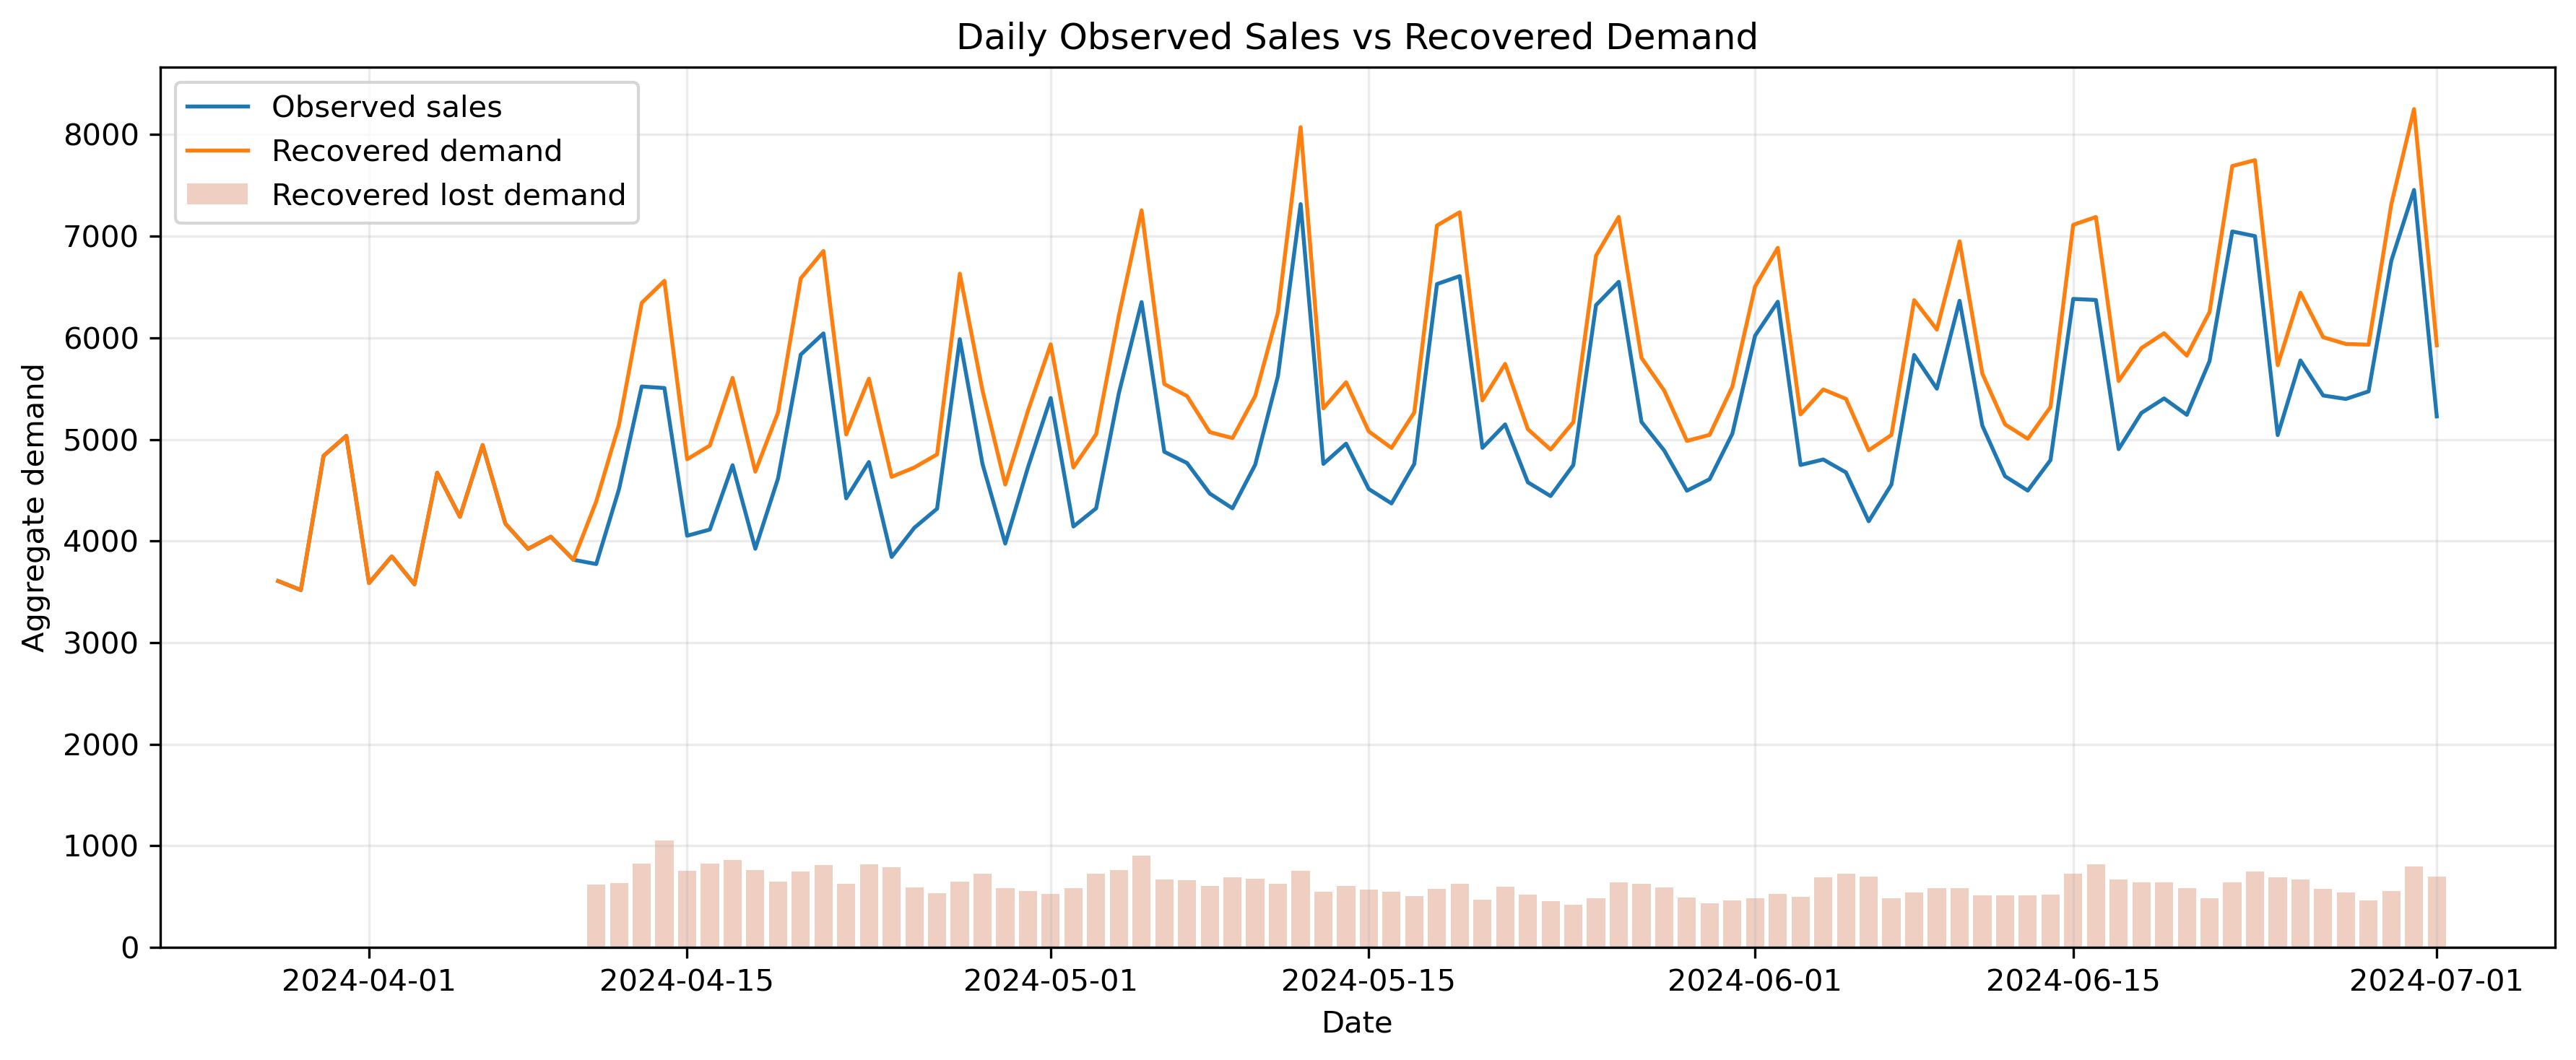
\includegraphics[width=0.92\linewidth]{../figures/imputation_daily_uplift.png}
    \caption{Observed sales, recovered demand và phần lost demand recovered theo ngày.}
    \label{fig:vi-imputation-daily-uplift}
\end{figure}


\begin{figure}[H]
    \centering
    
\includegraphics[width=0.78\linewidth]{../figures/imputation_series_lift_distribution.png}
    \caption{Phân phối recovered lift ở cấp series.}
    \label{fig:vi-imputation-lift-dist}
\end{figure}


\begin{figure}[H]
    \centering
    
\includegraphics[width=0.78\linewidth]{../figures/imputation_top_series_lift.png}
    \caption{Top series có recovered lift cao nhất.}
    \label{fig:vi-imputation-top-series}
\end{figure}


\begin{table}[H]
\centering
\caption{Top series phụ thuộc nhiều nhất vào imputation}
\resizebox{\linewidth}{!}{%
\begin{tabular}{lllllll}
\toprule
series\_id & observed\_sales & recovered\_demand & recovered\_lost\_demand & stockout\_rate & Recovered lift over observed & Recovered share from imputation \\
\midrule
0\_554\_90 & 39.3000 & 72.3776 & 33.0776 & 0.7339 & 0.8417 & 0.4570 \\
0\_597\_41 & 39.8500 & 71.9541 & 32.1041 & 0.6150 & 0.8056 & 0.4462 \\
3\_724\_188 & 45.3000 & 76.9671 & 31.6671 & 0.7248 & 0.6991 & 0.4114 \\
4\_356\_90 & 39.0500 & 66.2217 & 27.1717 & 0.6029 & 0.6958 & 0.4103 \\
11\_533\_129 & 43.7000 & 72.7158 & 29.0158 & 0.7161 & 0.6640 & 0.3990 \\
6\_493\_129 & 44.2000 & 73.4980 & 29.2980 & 0.7357 & 0.6629 & 0.3986 \\
0\_173\_90 & 55.3000 & 91.7408 & 36.4408 & 0.6536 & 0.6590 & 0.3972 \\
5\_6\_757 & 44.5000 & 72.8119 & 28.3119 & 0.7448 & 0.6362 & 0.3888 \\
12\_228\_129 & 45.7000 & 74.0857 & 28.3857 & 0.6667 & 0.6211 & 0.3831 \\
3\_835\_333 & 46.7000 & 74.9063 & 28.2063 & 0.6944 & 0.6040 & 0.3766 \\
\bottomrule
\end{tabular}
}
\end{table}

\begin{table}[H]
\centering
\caption{So sánh forecast trên observed sales và recovered demand}
\resizebox{\linewidth}{!}{%
\begin{tabular}{lllllllll}
\toprule
Model & Training target & Evaluation target & RMSE & MAE & WAPE & sMAPE & WPE & N \\
\midrule
Recovered naive x7 & baseline\_no\_training & Recovered latent demand proxy & 4.3949 & 2.8080 & 0.3149 & 0.3870 & -0.0198 & 70000 \\
Recovered seasonal naive 7-day & baseline\_no\_training & Recovered latent demand proxy & 2.9113 & 1.7704 & 0.1985 & 0.2269 & -0.0614 & 70000 \\
Recovered rolling mean 14-day & baseline\_no\_training & Recovered latent demand proxy & 3.1099 & 1.8367 & 0.2060 & 0.2268 & -0.0807 & 70000 \\
Observed-sales forecasting & target\_next7\_observed\_daily & Recovered latent demand proxy & 3.6749 & 2.1780 & 0.2442 & 0.2755 & -0.1788 & 70000 \\
Observed-sales forecasting & target\_next7\_observed\_daily & Observed sales & 3.2644 & 1.7730 & 0.2206 & 0.2412 & -0.0887 & 70000 \\
Recovered-demand forecasting & target\_next7\_recovered\_daily & Recovered latent demand proxy & 3.6160 & 1.8082 & 0.2028 & 0.2135 & -0.0800 & 70000 \\
Recovered-demand forecasting & target\_next7\_recovered\_daily & Observed sales & 3.4820 & 1.7713 & 0.2204 & 0.2459 & 0.0209 & 70000 \\
Recovered seasonal-ML hybrid & seasonal\_naive\_plus\_recovered\_lightgbm\_alpha\_0.60 & Recovered latent demand proxy & 3.2106 & 1.7545 & 0.1967 & 0.2127 & -0.0726 & 70000 \\
\bottomrule
\end{tabular}
}
\end{table}


\begin{figure}[H]
    \centering
    
\includegraphics[width=0.82\linewidth]{../figures/owner_two_stage_bias_comparison.png}
    \caption{So sánh bias WPE khi đánh giá trên recovered latent demand proxy.}
    \label{fig:vi-owner-bias}
\end{figure}


\begin{figure}[H]
    \centering
    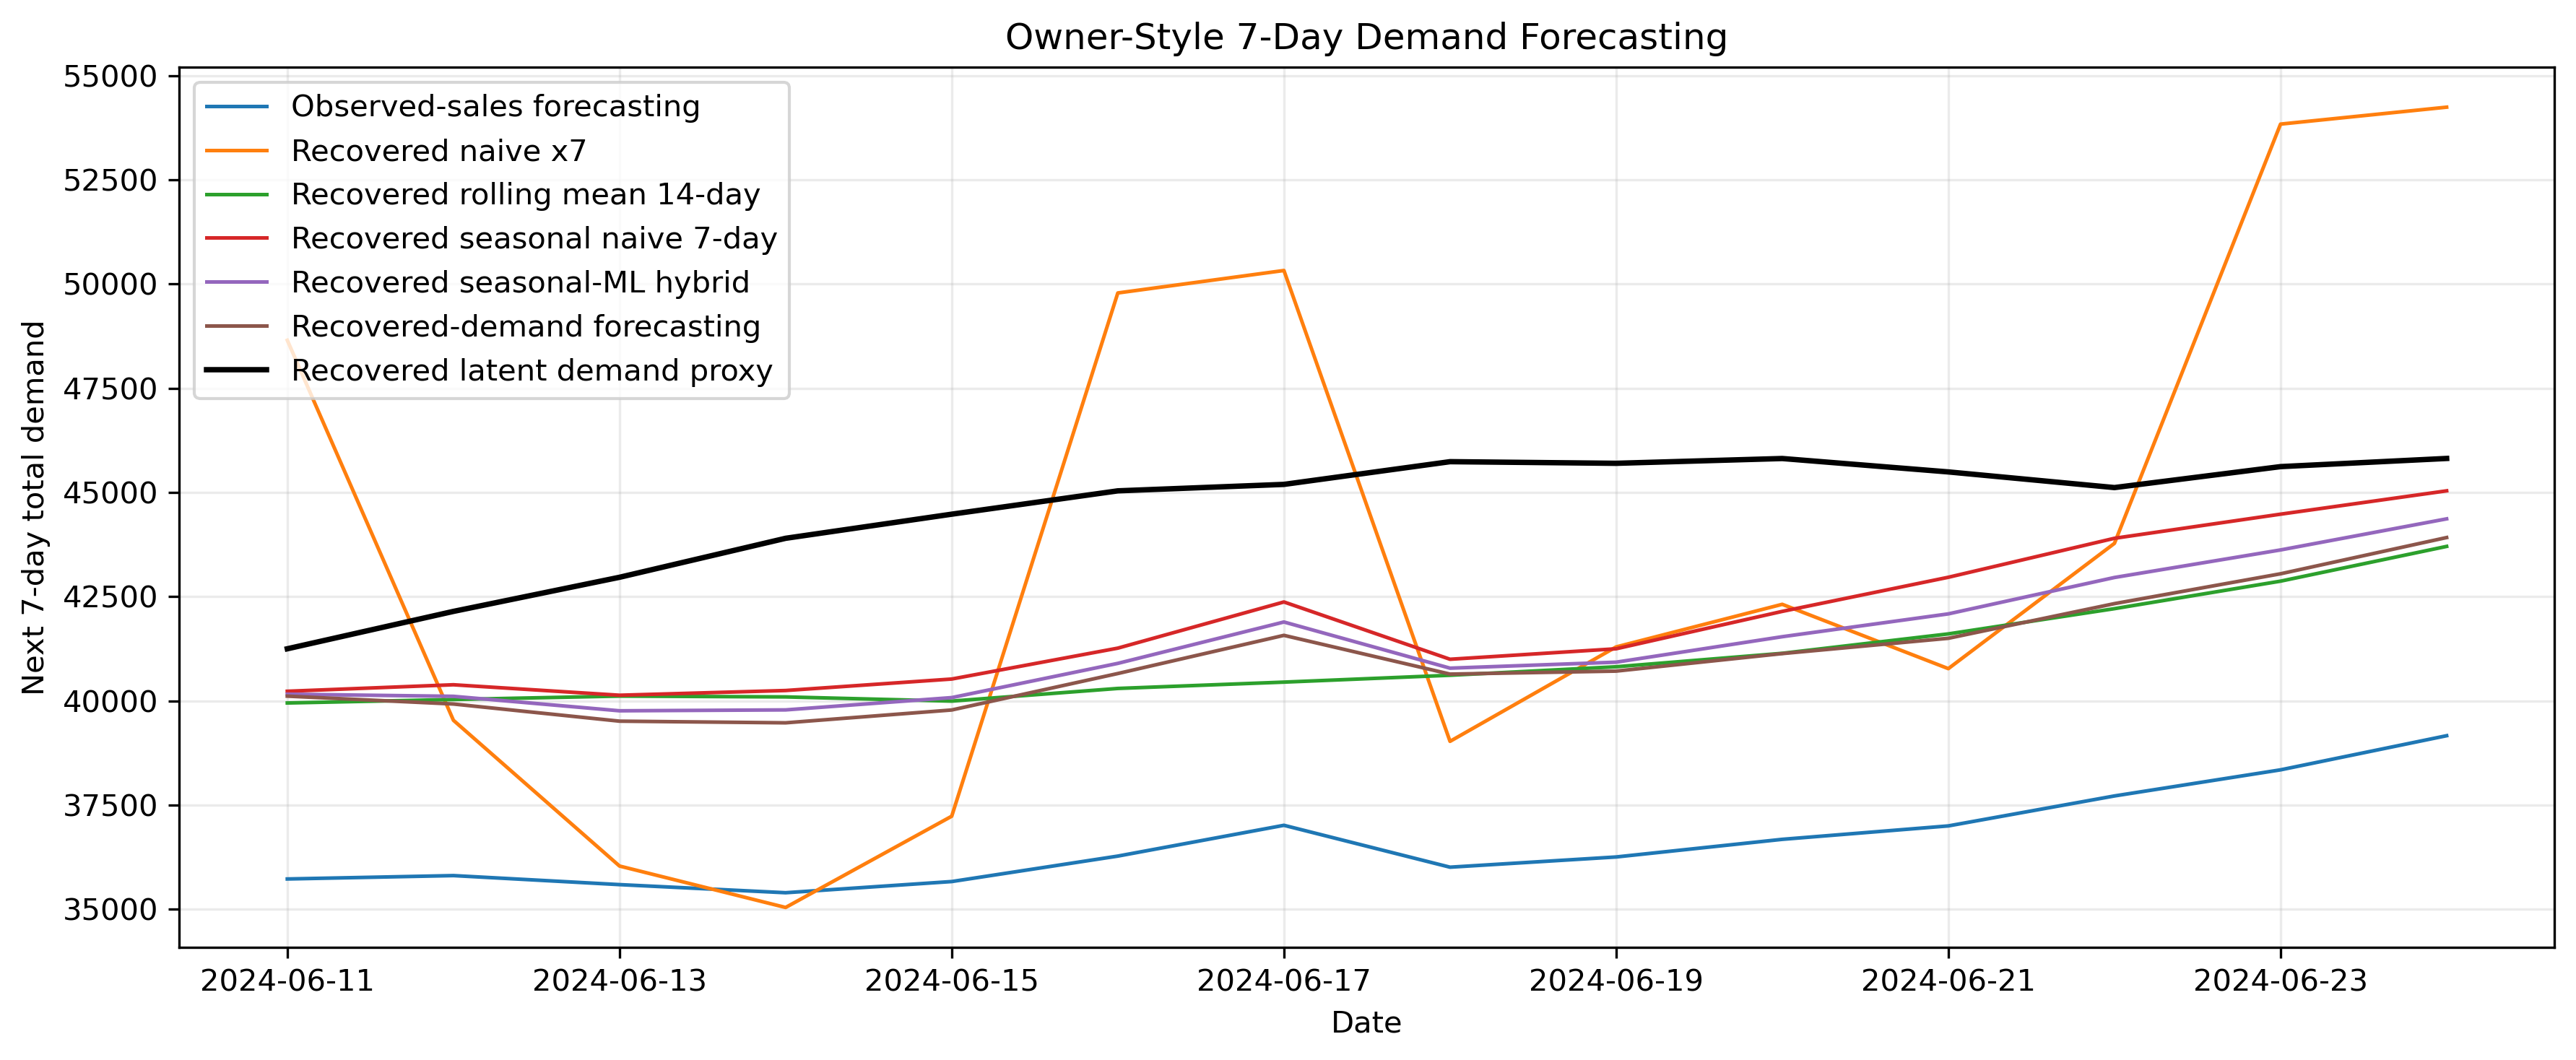
\includegraphics[width=0.92\linewidth]{../figures/owner_two_stage_forecast_comparison.png}
    \caption{Dự báo tổng nhu cầu 7 ngày theo hướng two-stage.}
    \label{fig:vi-owner-forecast}
\end{figure}


\section{Kết quả mô hình two-stage}
Sau khi khôi phục latent demand, phần dự báo chính của đồ án không còn xem observed sales là target cuối cùng.
Target chính là \texttt{target\_next7\_recovered\_daily}, tức tổng nhu cầu 7 ngày tiếp theo sau khi đã hiệu chỉnh các giờ stockout.
Để chứng minh lợi ích của two-stage, ta so sánh hai mô hình LightGBM có cùng dạng global model:
\begin{enumerate}
    \item \textbf{Observed-sales forecasting}: train trên doanh số quan sát được, sau đó đánh giá lại trên recovered latent demand proxy.
    \item \textbf{Recovered-demand forecasting}: train trực tiếp trên recovered demand và đánh giá trên recovered latent demand proxy.
\end{enumerate}
Ngoài ra, báo cáo thêm các baseline daily không cần train như naive, seasonal naive 7 ngày và rolling mean 14 ngày.
Seasonal naive 7 ngày là baseline rất mạnh vì phổ tần số và ACF đều cho thấy seasonality theo tuần.
Mô hình cuối cùng được dùng để kết luận là \textbf{Recovered seasonal-ML hybrid}: blend giữa seasonal naive 7 ngày và Recovered-demand LightGBM, với trọng số được chọn trên validation set.
Cách này giữ được nền mùa vụ mạnh của seasonal naive, đồng thời cho phép LightGBM hiệu chỉnh theo stockout, lag, rolling và calendar features.

\begin{table}[H]
\centering
\caption{Kết quả chính của mô hình two-stage}
\resizebox{\linewidth}{!}{%
\begin{tabular}{lllllllll}
\toprule
Model & Training target & Evaluation target & RMSE & MAE & WAPE & sMAPE & WPE & N \\
\midrule
Recovered naive x7 & baseline\_no\_training & Recovered latent demand proxy & 4.3949 & 2.8080 & 0.3149 & 0.3870 & -0.0198 & 70000 \\
Recovered seasonal naive 7-day & baseline\_no\_training & Recovered latent demand proxy & 2.9113 & 1.7704 & 0.1985 & 0.2269 & -0.0614 & 70000 \\
Recovered rolling mean 14-day & baseline\_no\_training & Recovered latent demand proxy & 3.1099 & 1.8367 & 0.2060 & 0.2268 & -0.0807 & 70000 \\
Observed-sales forecasting & target\_next7\_observed\_daily & Recovered latent demand proxy & 3.6749 & 2.1780 & 0.2442 & 0.2755 & -0.1788 & 70000 \\
Observed-sales forecasting & target\_next7\_observed\_daily & Observed sales & 3.2644 & 1.7730 & 0.2206 & 0.2412 & -0.0887 & 70000 \\
Recovered-demand forecasting & target\_next7\_recovered\_daily & Recovered latent demand proxy & 3.6160 & 1.8082 & 0.2028 & 0.2135 & -0.0800 & 70000 \\
Recovered-demand forecasting & target\_next7\_recovered\_daily & Observed sales & 3.4820 & 1.7713 & 0.2204 & 0.2459 & 0.0209 & 70000 \\
Recovered seasonal-ML hybrid & seasonal\_naive\_plus\_recovered\_lightgbm\_alpha\_0.60 & Recovered latent demand proxy & 3.2106 & 1.7545 & 0.1967 & 0.2127 & -0.0726 & 70000 \\
\bottomrule
\end{tabular}
}
\end{table}

Kết quả cho thấy train trên recovered demand làm giảm sai số khi đánh giá trên recovered latent demand proxy, đồng thời làm bias âm nhỏ hơn.
Điều này quan trọng vì mô hình train trên observed sales có xu hướng under-forecast nhu cầu trong các giai đoạn từng bị stockout.
Baseline seasonal naive 7 ngày cũng rất cạnh tranh, cho thấy tính mùa vụ tuần là pattern chính của dữ liệu.
Hybrid seasonal-ML đạt WAPE 0.1967, là kết quả tốt nhất trong bảng, nên được dùng làm mô hình kết luận cuối.

\begin{table}[H]
\centering
\caption{Chọn trọng số hybrid trên validation set}
\resizebox{0.72\linewidth}{!}{%
\begin{tabular}{lll}
\toprule
LightGBM weight & Seasonal naive weight & Validation WAPE \\
\midrule
0.6000 & 0.4000 & 0.1901 \\
0.5500 & 0.4500 & 0.1901 \\
0.6500 & 0.3500 & 0.1902 \\
0.5000 & 0.5000 & 0.1903 \\
0.7000 & 0.3000 & 0.1903 \\
0.4500 & 0.5500 & 0.1906 \\
0.7500 & 0.2500 & 0.1906 \\
0.4000 & 0.6000 & 0.1909 \\
\bottomrule
\end{tabular}
}
\end{table}


\begin{figure}[H]
    \centering
    
\includegraphics[width=0.82\linewidth]{../figures/owner_two_stage_bias_comparison.png}
    \caption{Bias WPE của mô hình observed-sales và recovered-demand khi đánh giá trên recovered latent demand proxy.}
    \label{fig:vi-owner-bias-main}
\end{figure}


\begin{figure}[H]
    \centering
    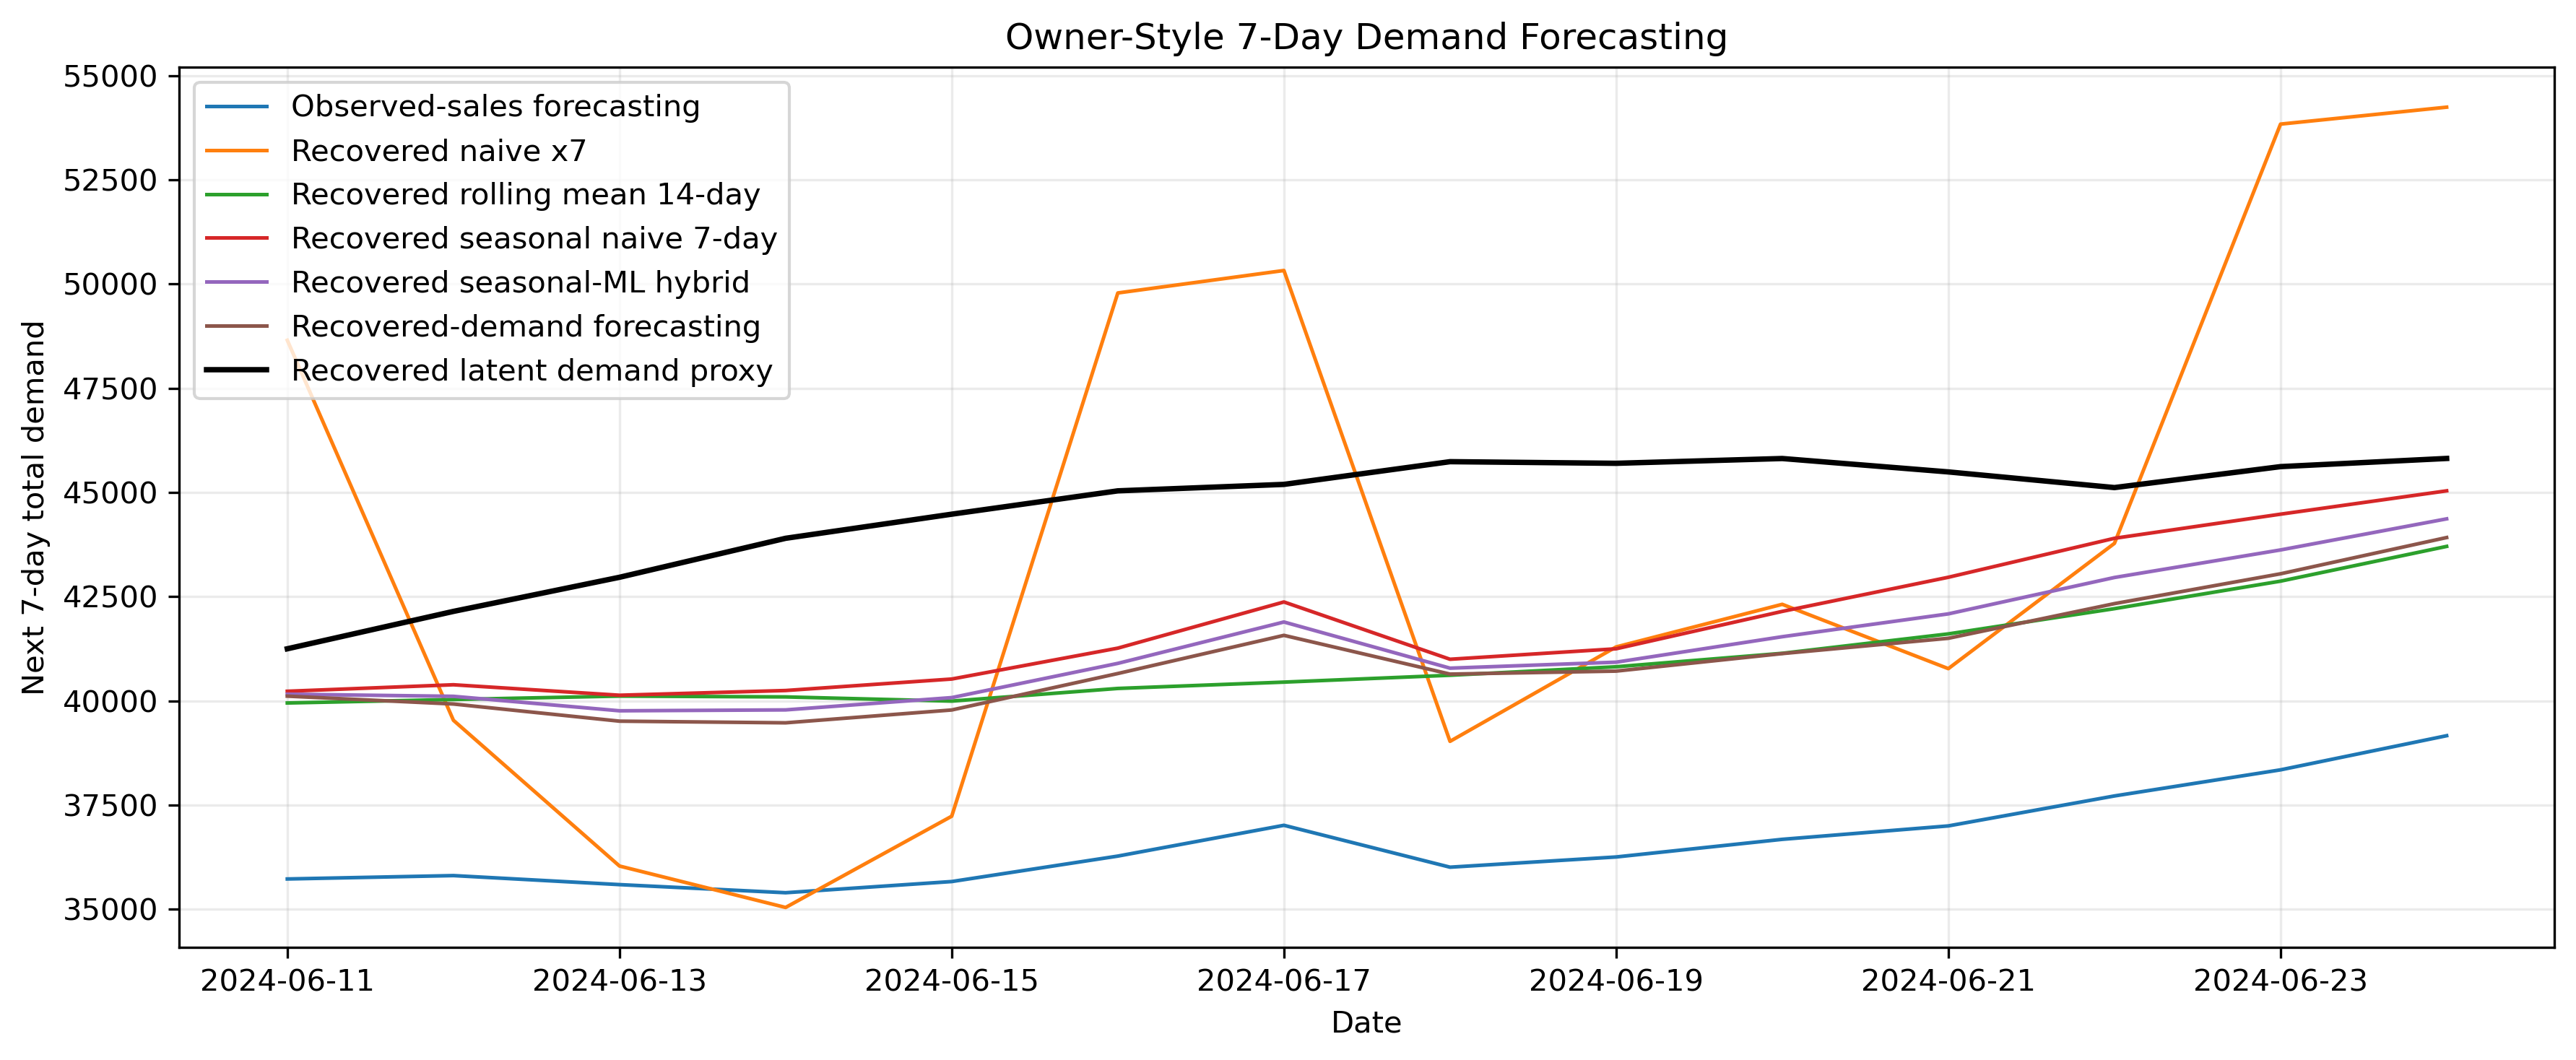
\includegraphics[width=0.92\linewidth]{../figures/owner_two_stage_forecast_comparison.png}
    \caption{Dự báo tổng nhu cầu 7 ngày theo hướng two-stage.}
    \label{fig:vi-owner-forecast-main}
\end{figure}


\subsection{Benchmark observed-sales hourly}
Các kết quả h=1 và h=24 trên observed sales vẫn được giữ như benchmark phụ để cho thấy pipeline feature engineering và LightGBM hourly hoạt động hợp lý.
Tuy nhiên, chúng không còn là kết quả chính vì observed sales bị kiểm duyệt trong các giờ stockout.

\begin{table}[H]
\centering
\caption{Benchmark phụ trên observed sales cho horizon h=1}
\begin{tabular}{llllll}
\toprule
Model & RMSE & MAE & WAPE & sMAPE & N \\
\midrule
LightGBM & 0.0957 & 0.0513 & 1.0483 & 1.7028 & 1680000 \\
Ridge & 0.1019 & 0.0546 & 1.1141 & 1.7237 & 1680000 \\
SeasonalNaive168 & 0.1323 & 0.0588 & 1.2007 & 0.5970 & 1680000 \\
SeasonalNaive24 & 0.1367 & 0.0601 & 1.2260 & 0.5991 & 1680000 \\
Naive & 0.1414 & 0.0609 & 1.2441 & 0.5973 & 1680000 \\
\bottomrule
\end{tabular}
\end{table}

\begin{table}[H]
\centering
\caption{Benchmark phụ trên observed sales cho horizon h=24}
\begin{tabular}{llllll}
\toprule
Model & RMSE & MAE & WAPE & sMAPE & N \\
\midrule
LightGBM & 0.0986 & 0.0525 & 1.0695 & 1.7195 & 1680000 \\
Ridge & 0.1025 & 0.0573 & 1.1663 & 1.7113 & 1680000 \\
SeasonalNaive168 & 0.1314 & 0.0582 & 1.1837 & 0.5913 & 1680000 \\
Naive & 0.1350 & 0.0594 & 1.2094 & 0.5943 & 1680000 \\
SeasonalNaive24 & 0.1350 & 0.0594 & 1.2094 & 0.5943 & 1680000 \\
\bottomrule
\end{tabular}
\end{table}

\section{Diagnostics và khoảng dự báo two-stage}
Diagnostics chính được thực hiện trên mô hình \textbf{Recovered seasonal-ML hybrid}, với residual được tính theo recovered latent demand proxy.
Cách đánh giá này nhất quán với mục tiêu của two-stage: sau khi hiệu chỉnh latent demand, mô hình phải dự báo nhu cầu đã khử kiểm duyệt, không chỉ dự báo observed sales.
Bảng dưới đây vẫn hiển thị cả baseline, observed-sales, recovered-demand và hybrid để so sánh trực tiếp, nhưng diễn giải chính tập trung vào mô hình có WAPE thấp nhất trên recovered latent demand proxy.

\begin{table}[H]
\centering
\caption{Diagnostics của mô hình two-stage trên recovered latent demand proxy}
\resizebox{\linewidth}{!}{%
\begin{tabular}{llllllllllll}
\toprule
Model & Evaluation target & RMSE & MAE & WAPE & sMAPE & WPE & Residual mean & Residual std & Ljung-Box p-value & Jarque-Bera p-value & N \\
\midrule
Recovered naive x7 & Recovered latent demand proxy & 4.3949 & 2.8080 & 0.3149 & 0.3870 & -0.0198 & 0.1770 & 4.3913 & 0.1790 & 0.0000 & 70000 \\
Recovered seasonal naive 7-day & Recovered latent demand proxy & 2.9113 & 1.7704 & 0.1985 & 0.2269 & -0.0614 & 0.5475 & 2.8594 & 0.0131 & 0.0000 & 70000 \\
Recovered rolling mean 14-day & Recovered latent demand proxy & 3.1099 & 1.8367 & 0.2060 & 0.2268 & -0.0807 & 0.7194 & 3.0255 & 0.0001 & 0.0000 & 70000 \\
Observed-sales forecasting & Recovered latent demand proxy & 3.6749 & 2.1780 & 0.2442 & 0.2755 & -0.1788 & 1.5943 & 3.3111 & 0.0127 & 0.0000 & 70000 \\
Recovered-demand forecasting & Recovered latent demand proxy & 3.6160 & 1.8082 & 0.2028 & 0.2135 & -0.0800 & 0.7134 & 3.5450 & 0.0665 & 0.0000 & 70000 \\
Recovered seasonal-ML hybrid & Recovered latent demand proxy & 3.2106 & 1.7545 & 0.1967 & 0.2127 & -0.0726 & 0.6470 & 3.1448 & 0.0311 & 0.0000 & 70000 \\
\bottomrule
\end{tabular}
}
\end{table}


\begin{figure}[H]
    \centering
    
\includegraphics[width=0.78\linewidth]{../figures/owner_two_stage_residual_distribution.png}
    \caption{Phân phối residual của recovered-demand forecasting trên recovered latent demand proxy.}
    \label{fig:vi-owner-residual-dist}
\end{figure}


\begin{figure}[H]
    \centering
    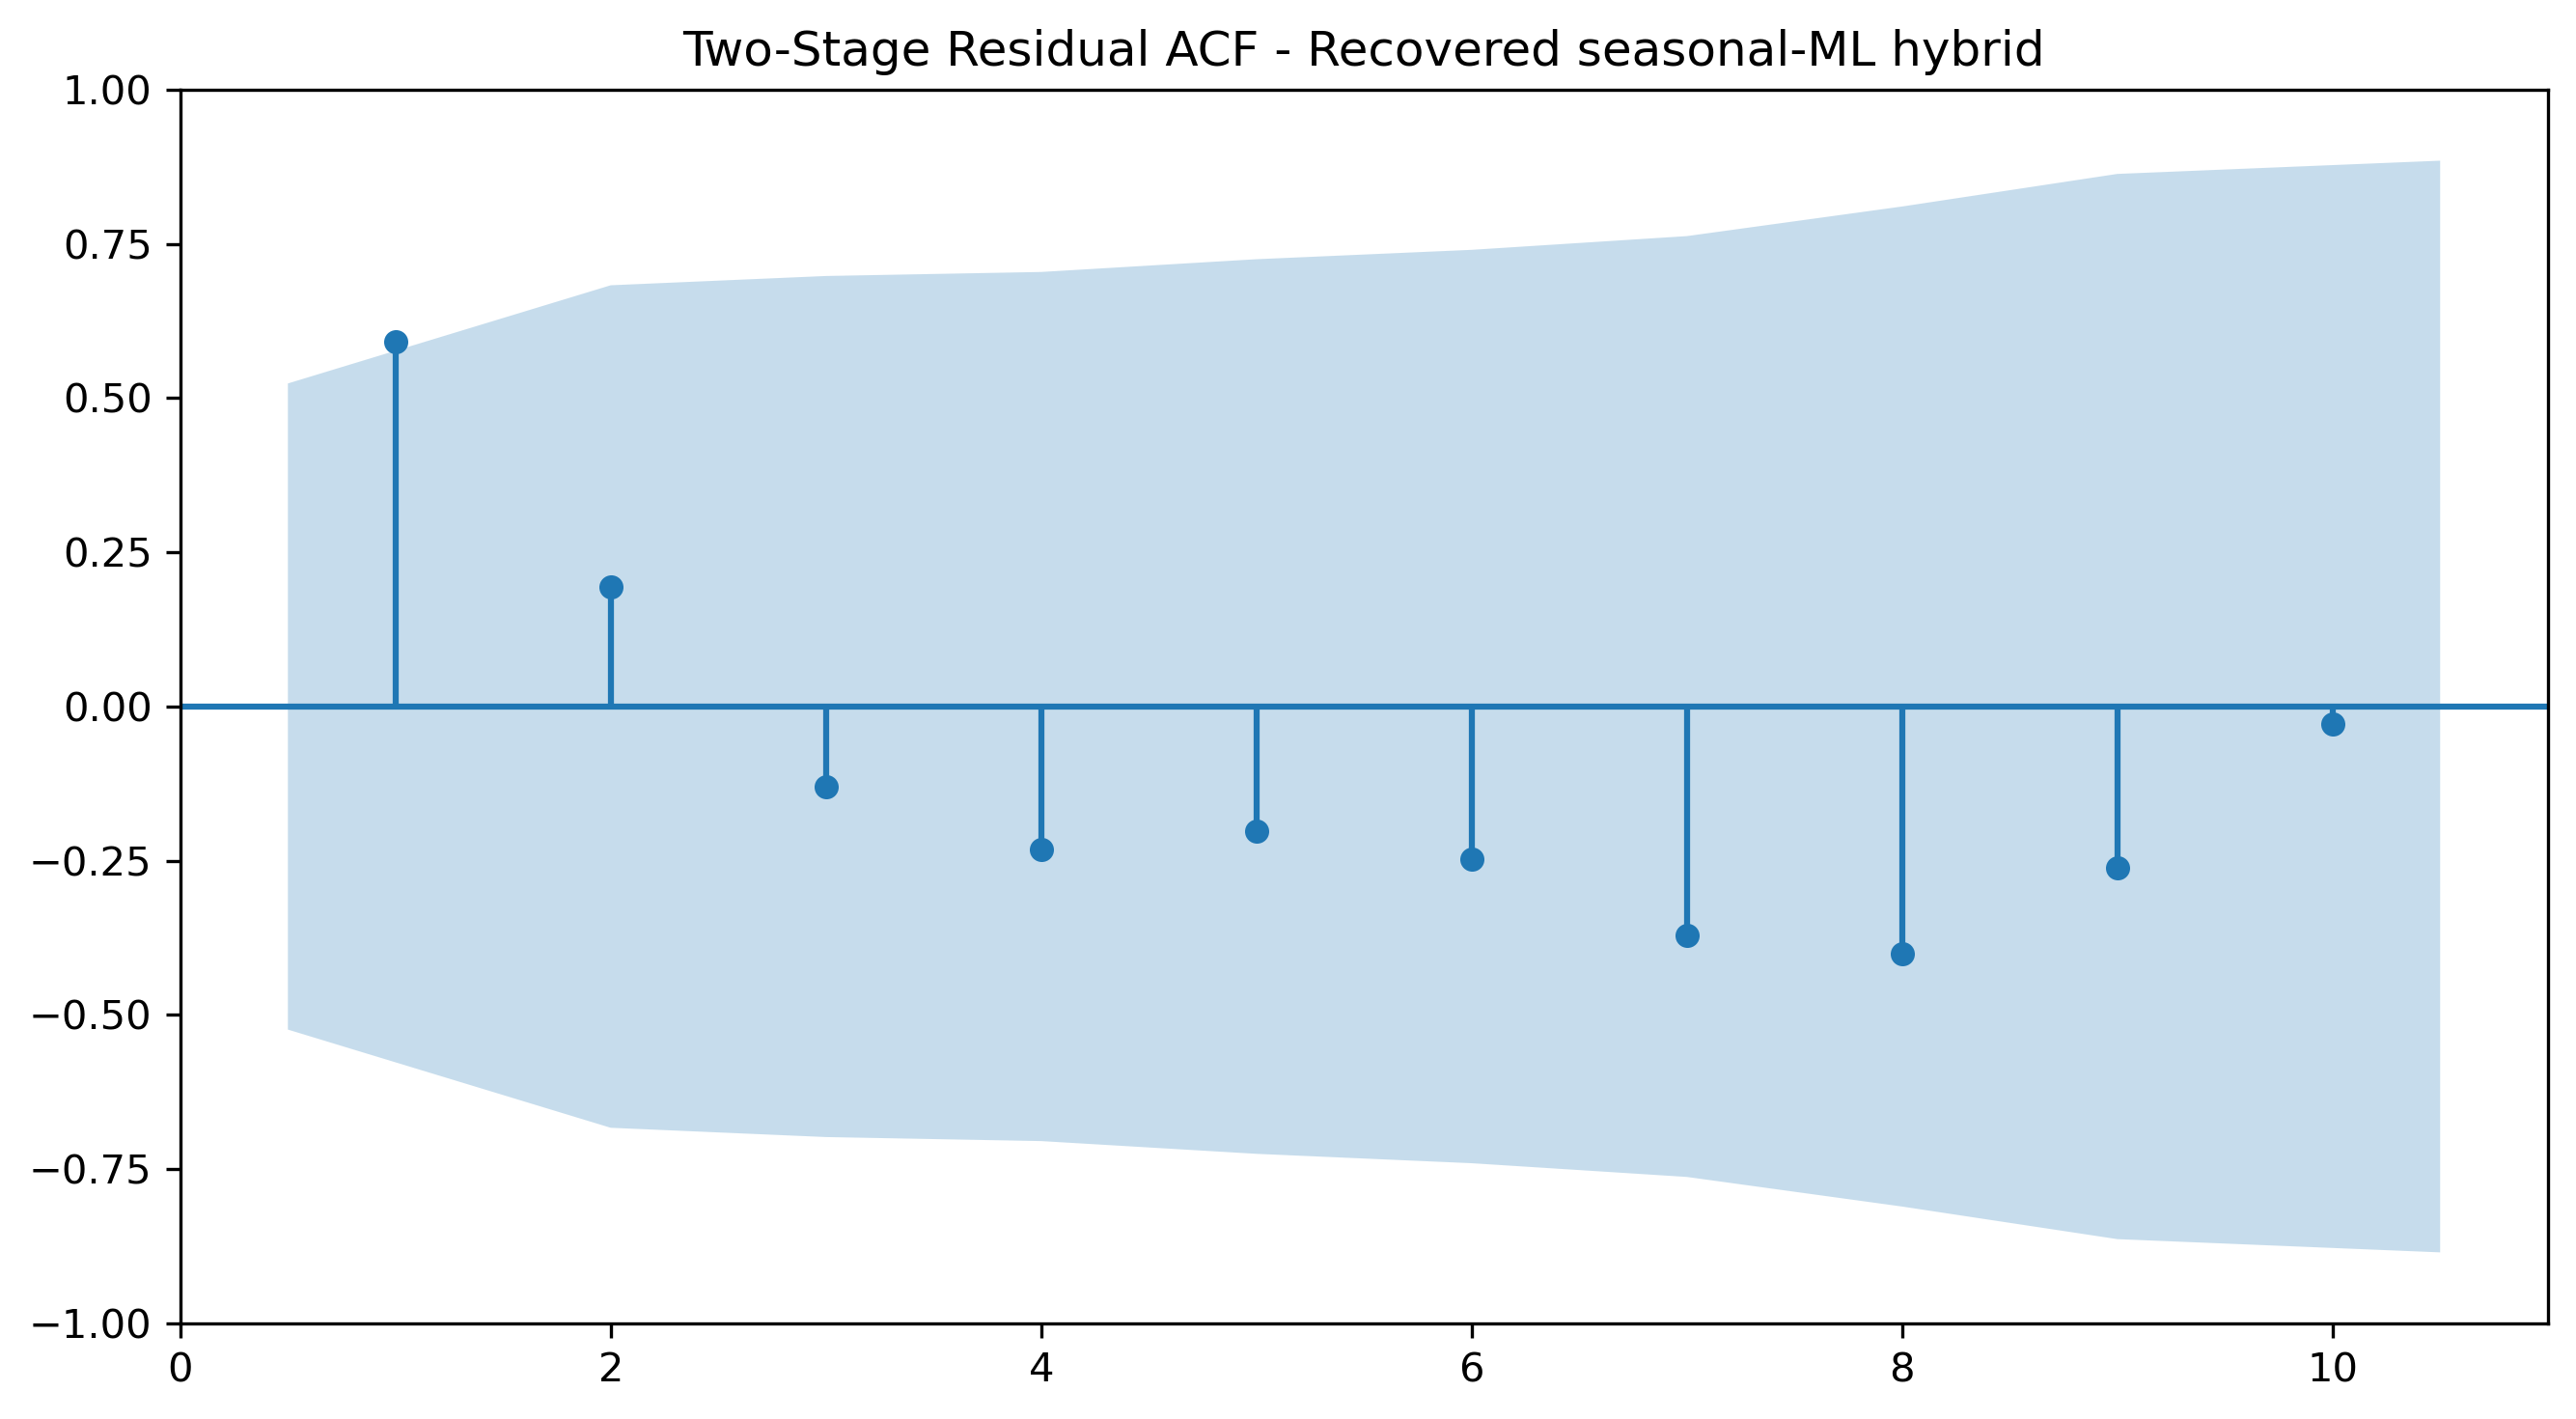
\includegraphics[width=0.82\linewidth]{../figures/owner_two_stage_residual_acf.png}
    \caption{Residual ACF của recovered-demand forecasting theo daily aggregate.}
    \label{fig:vi-owner-residual-acf}
\end{figure}


\begin{figure}[H]
    \centering
    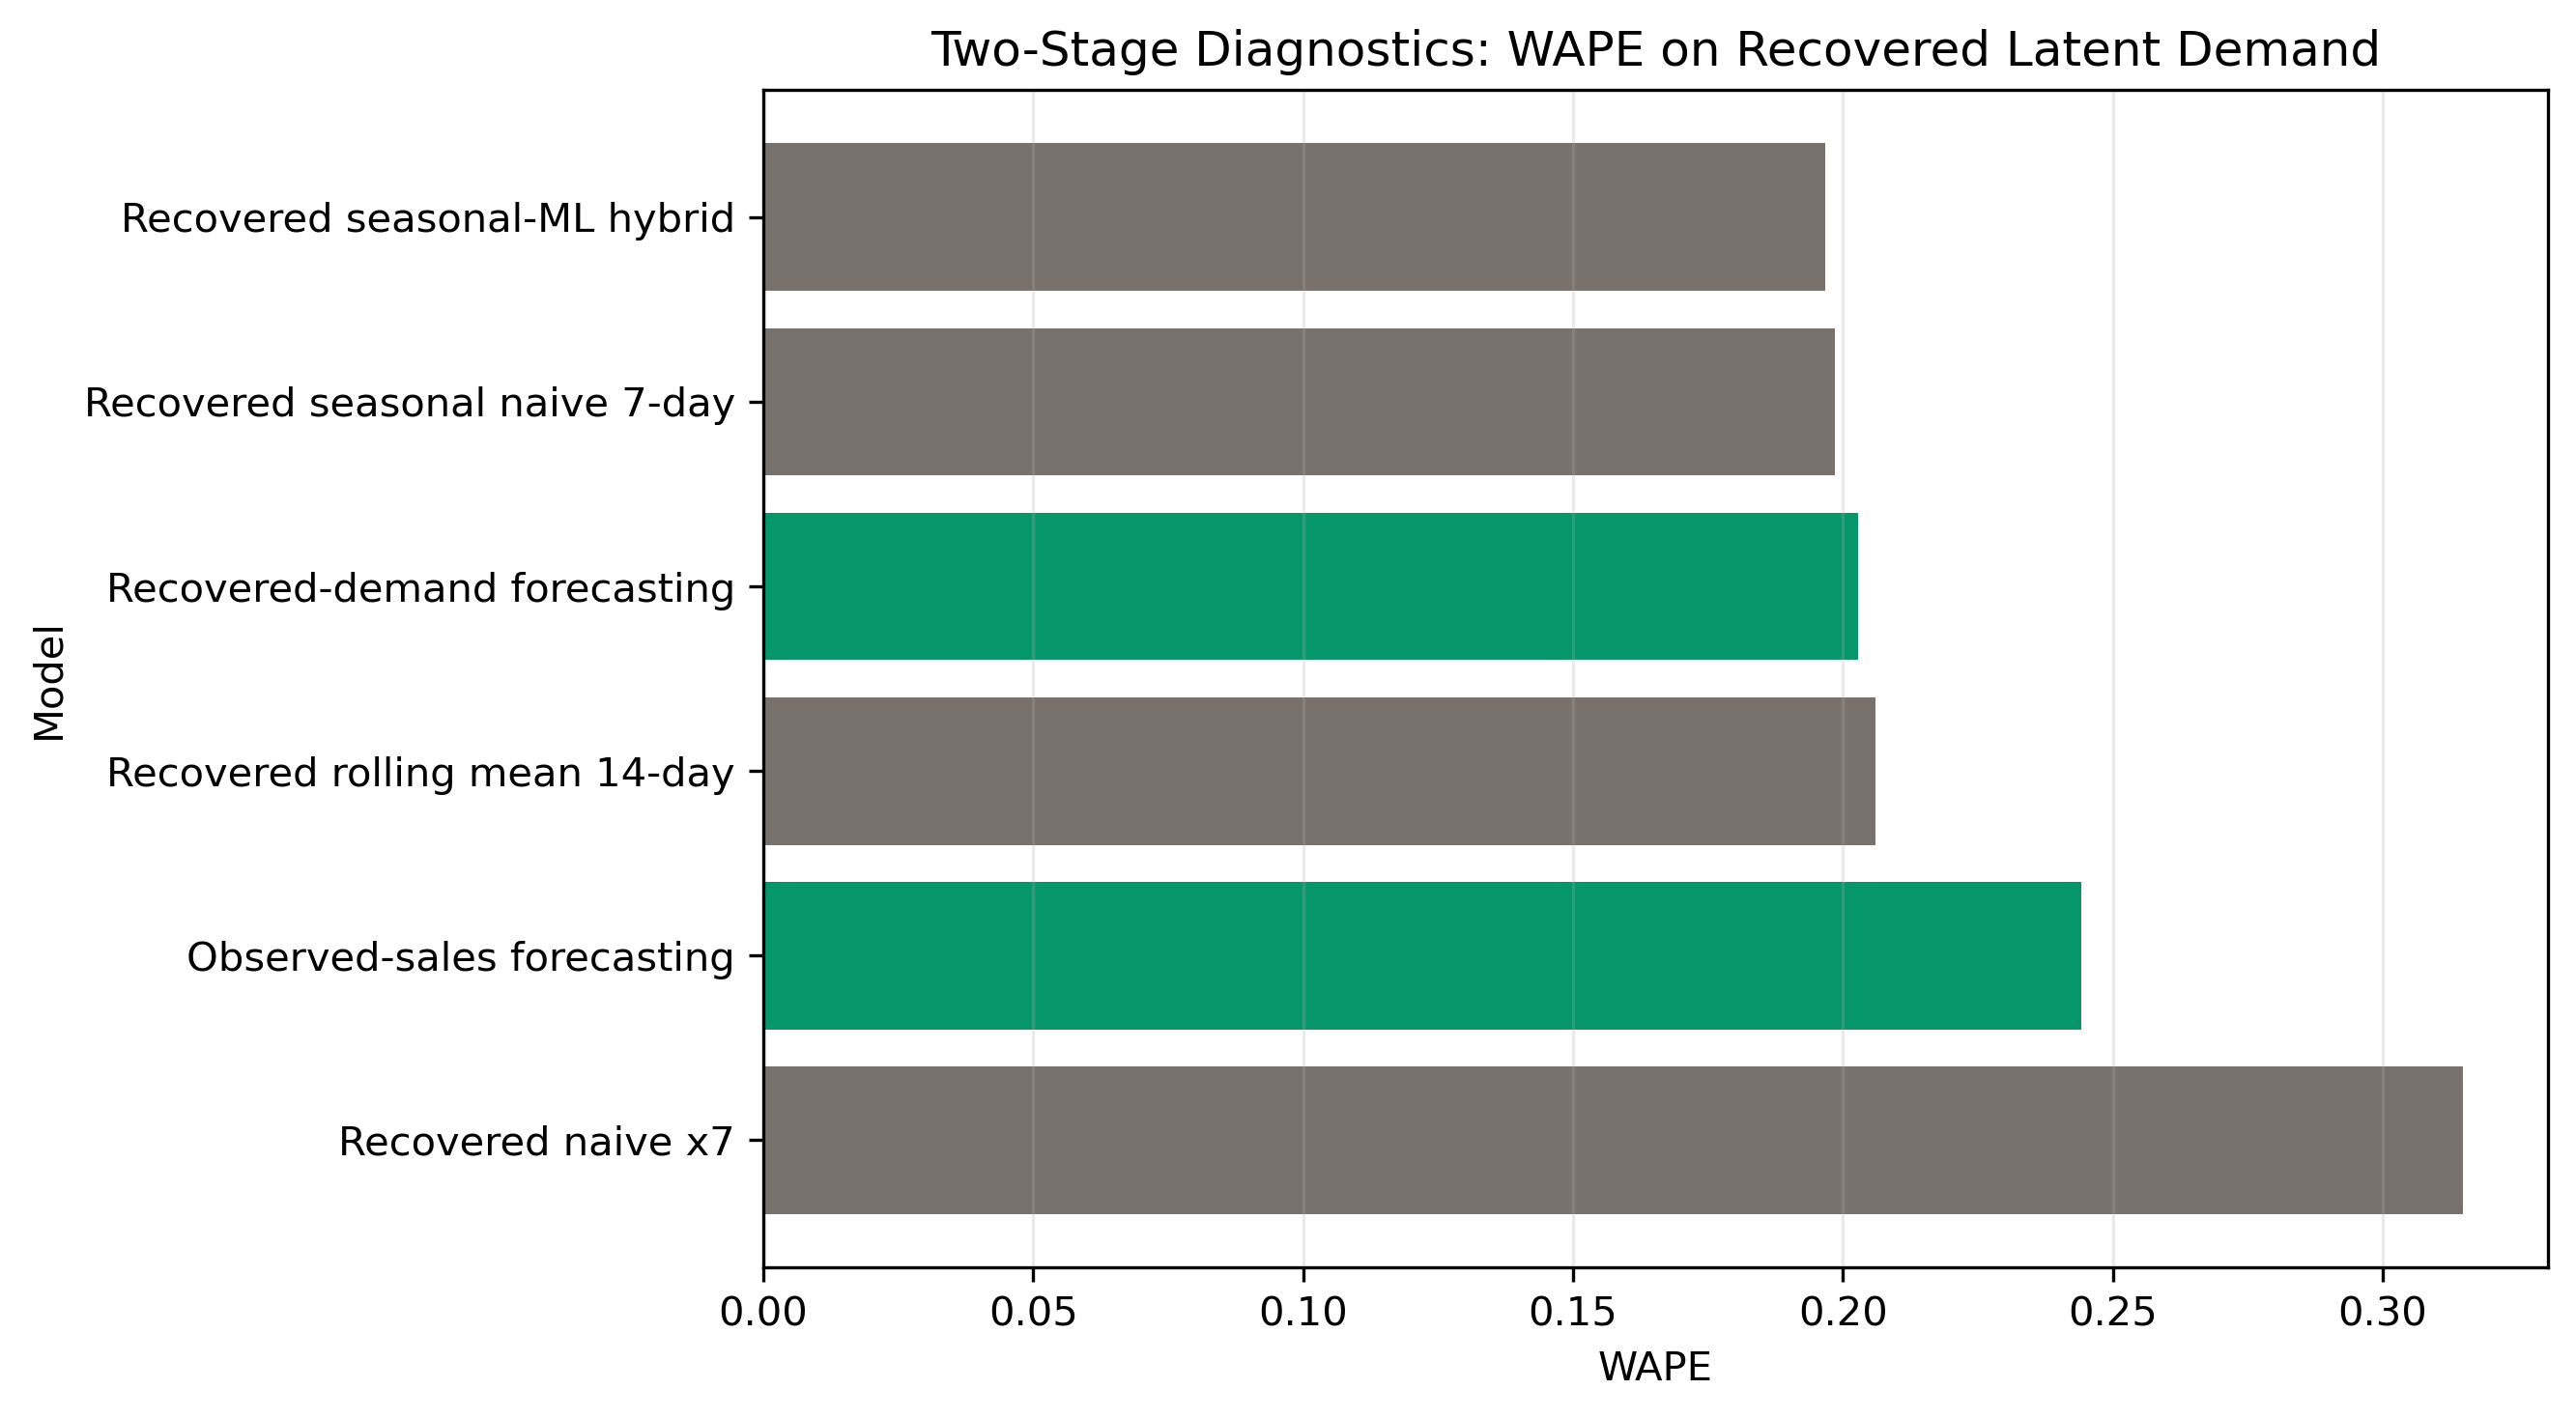
\includegraphics[width=0.78\linewidth]{../figures/owner_two_stage_diagnostics_wape.png}
    \caption{So sánh WAPE diagnostics của hai hướng train khi đánh giá trên recovered latent demand proxy.}
    \label{fig:vi-owner-diagnostics-wape}
\end{figure}


Vì target của bài toán là tổng nhu cầu 7 ngày tiếp theo, các nhãn dự báo theo từng ngày bị overlap mạnh: forecast tại ngày $t$ và ngày $t+1$ chia sẻ 6/7 ngày trong target.
Do đó, residual theo daily rolling evaluation có thể tự tương quan một phần do thiết kế target, không chỉ do mô hình học thiếu pattern.
Để kiểm tra độc lập residual công bằng hơn, báo cáo thêm diagnostics trên các mốc non-overlapping cách nhau 7 ngày.
Với Recovered seasonal-ML hybrid, diagnostics chính có Ljung--Box p-value 0.0311, tức vẫn còn tự tương quan nhẹ ở mức 5\% nếu đánh giá trên rolling target bị overlap.
Diagnostics non-overlapping có Ljung--Box p-value 0.1573, nên không bác bỏ tự tương quan ở mức 5\% trong kiểm tra phụ.
Tuy nhiên, do test set chỉ có 14 ngày nên non-overlapping aggregate chỉ có hai mốc thời gian; kết quả này được dùng như kiểm tra phụ, không phải bằng chứng tuyệt đối.

\begin{table}[H]
\centering
\caption{Diagnostics trên non-overlapping 7-day targets}
\resizebox{\linewidth}{!}{%
\begin{tabular}{llllllllll}
\toprule
Model & Evaluation mode & Evaluation dates & RMSE & MAE & WAPE & WPE & Ljung-Box p-value & N & Aggregate residual points \\
\midrule
Recovered naive x7 & Non-overlapping 7-day targets & 2024-06-11; 2024-06-18 & 4.6707 & 2.9483 & 0.3389 & 0.0080 & 0.1573 & 10000 & 2 \\
Recovered seasonal naive 7-day & Non-overlapping 7-day targets & 2024-06-11; 2024-06-18 & 2.8150 & 1.7140 & 0.1970 & -0.0662 & 0.1573 & 10000 & 2 \\
Recovered rolling mean 14-day & Non-overlapping 7-day targets & 2024-06-11; 2024-06-18 & 3.0150 & 1.7821 & 0.2049 & -0.0738 & 0.1573 & 10000 & 2 \\
Observed-sales forecasting & Non-overlapping 7-day targets & 2024-06-11; 2024-06-18 & 3.5320 & 2.1044 & 0.2419 & -0.1753 & 0.1573 & 10000 & 2 \\
Recovered-demand forecasting & Non-overlapping 7-day targets & 2024-06-11; 2024-06-18 & 3.3906 & 1.7544 & 0.2017 & -0.0716 & 0.1573 & 10000 & 2 \\
Recovered seasonal-ML hybrid & Non-overlapping 7-day targets & 2024-06-11; 2024-06-18 & 3.0564 & 1.7001 & 0.1954 & -0.0695 & 0.1573 & 10000 & 2 \\
\bottomrule
\end{tabular}
}
\end{table}

Khoảng dự báo được xây dựng từ phân vị residual trên validation set của mô hình two-stage.
Cách này không giả định residual phân phối chuẩn tuyệt đối, phù hợp hơn với dữ liệu bán lẻ thưa và có nhiều giá trị zero.


\begin{figure}[H]
    \centering
    
\includegraphics[width=0.92\linewidth]{../figures/owner_two_stage_forecast_interval.png}
    \caption{Khoảng dự báo 80\textbackslash\{\}\% và 95\textbackslash\{\}\% của mô hình two-stage trên recovered latent demand.}
    \label{fig:vi-owner-interval}
\end{figure}


\section{Diễn giải đặc trưng của mô hình two-stage}
Với hướng two-stage, feature importance chính được lấy từ mô hình \textbf{Recovered-demand forecasting} thay vì LightGBM hourly observed-sales.
Các đặc trưng quan trọng nhất chủ yếu là lag và rolling statistics của recovered demand, vì chúng mô tả mức nền nhu cầu sau khi đã hiệu chỉnh stockout.
Biến \texttt{stockout\_rate} vẫn được giữ trong mô hình forecasting để mô hình biết mức độ kiểm duyệt gần đây của chuỗi.

\begin{table}[H]
\centering
\caption{Top đặc trưng quan trọng của recovered-demand forecasting}
\begin{tabular}{ll}
\toprule
feature & importance \\
\midrule
stockout\_rate & 986 \\
recovered\_daily\_lag\_28 & 969 \\
recovered\_daily\_lag\_1 & 820 \\
recovered\_daily\_lag\_14 & 814 \\
recovered\_daily\_lag\_7 & 794 \\
recovered\_daily\_lag\_2 & 699 \\
recovered\_daily\_roll\_mean\_28 & 671 \\
recovered\_daily\_roll\_sum\_28 & 585 \\
day\_of\_week & 518 \\
recovered\_daily\_roll\_mean\_7 & 490 \\
month & 410 \\
recovered\_daily\_roll\_mean\_14 & 392 \\
recovered\_daily\_roll\_sum\_14 & 329 \\
recovered\_daily\_roll\_sum\_7 & 289 \\
is\_weekend & 23 \\
\bottomrule
\end{tabular}
\end{table}


\begin{figure}[H]
    \centering
    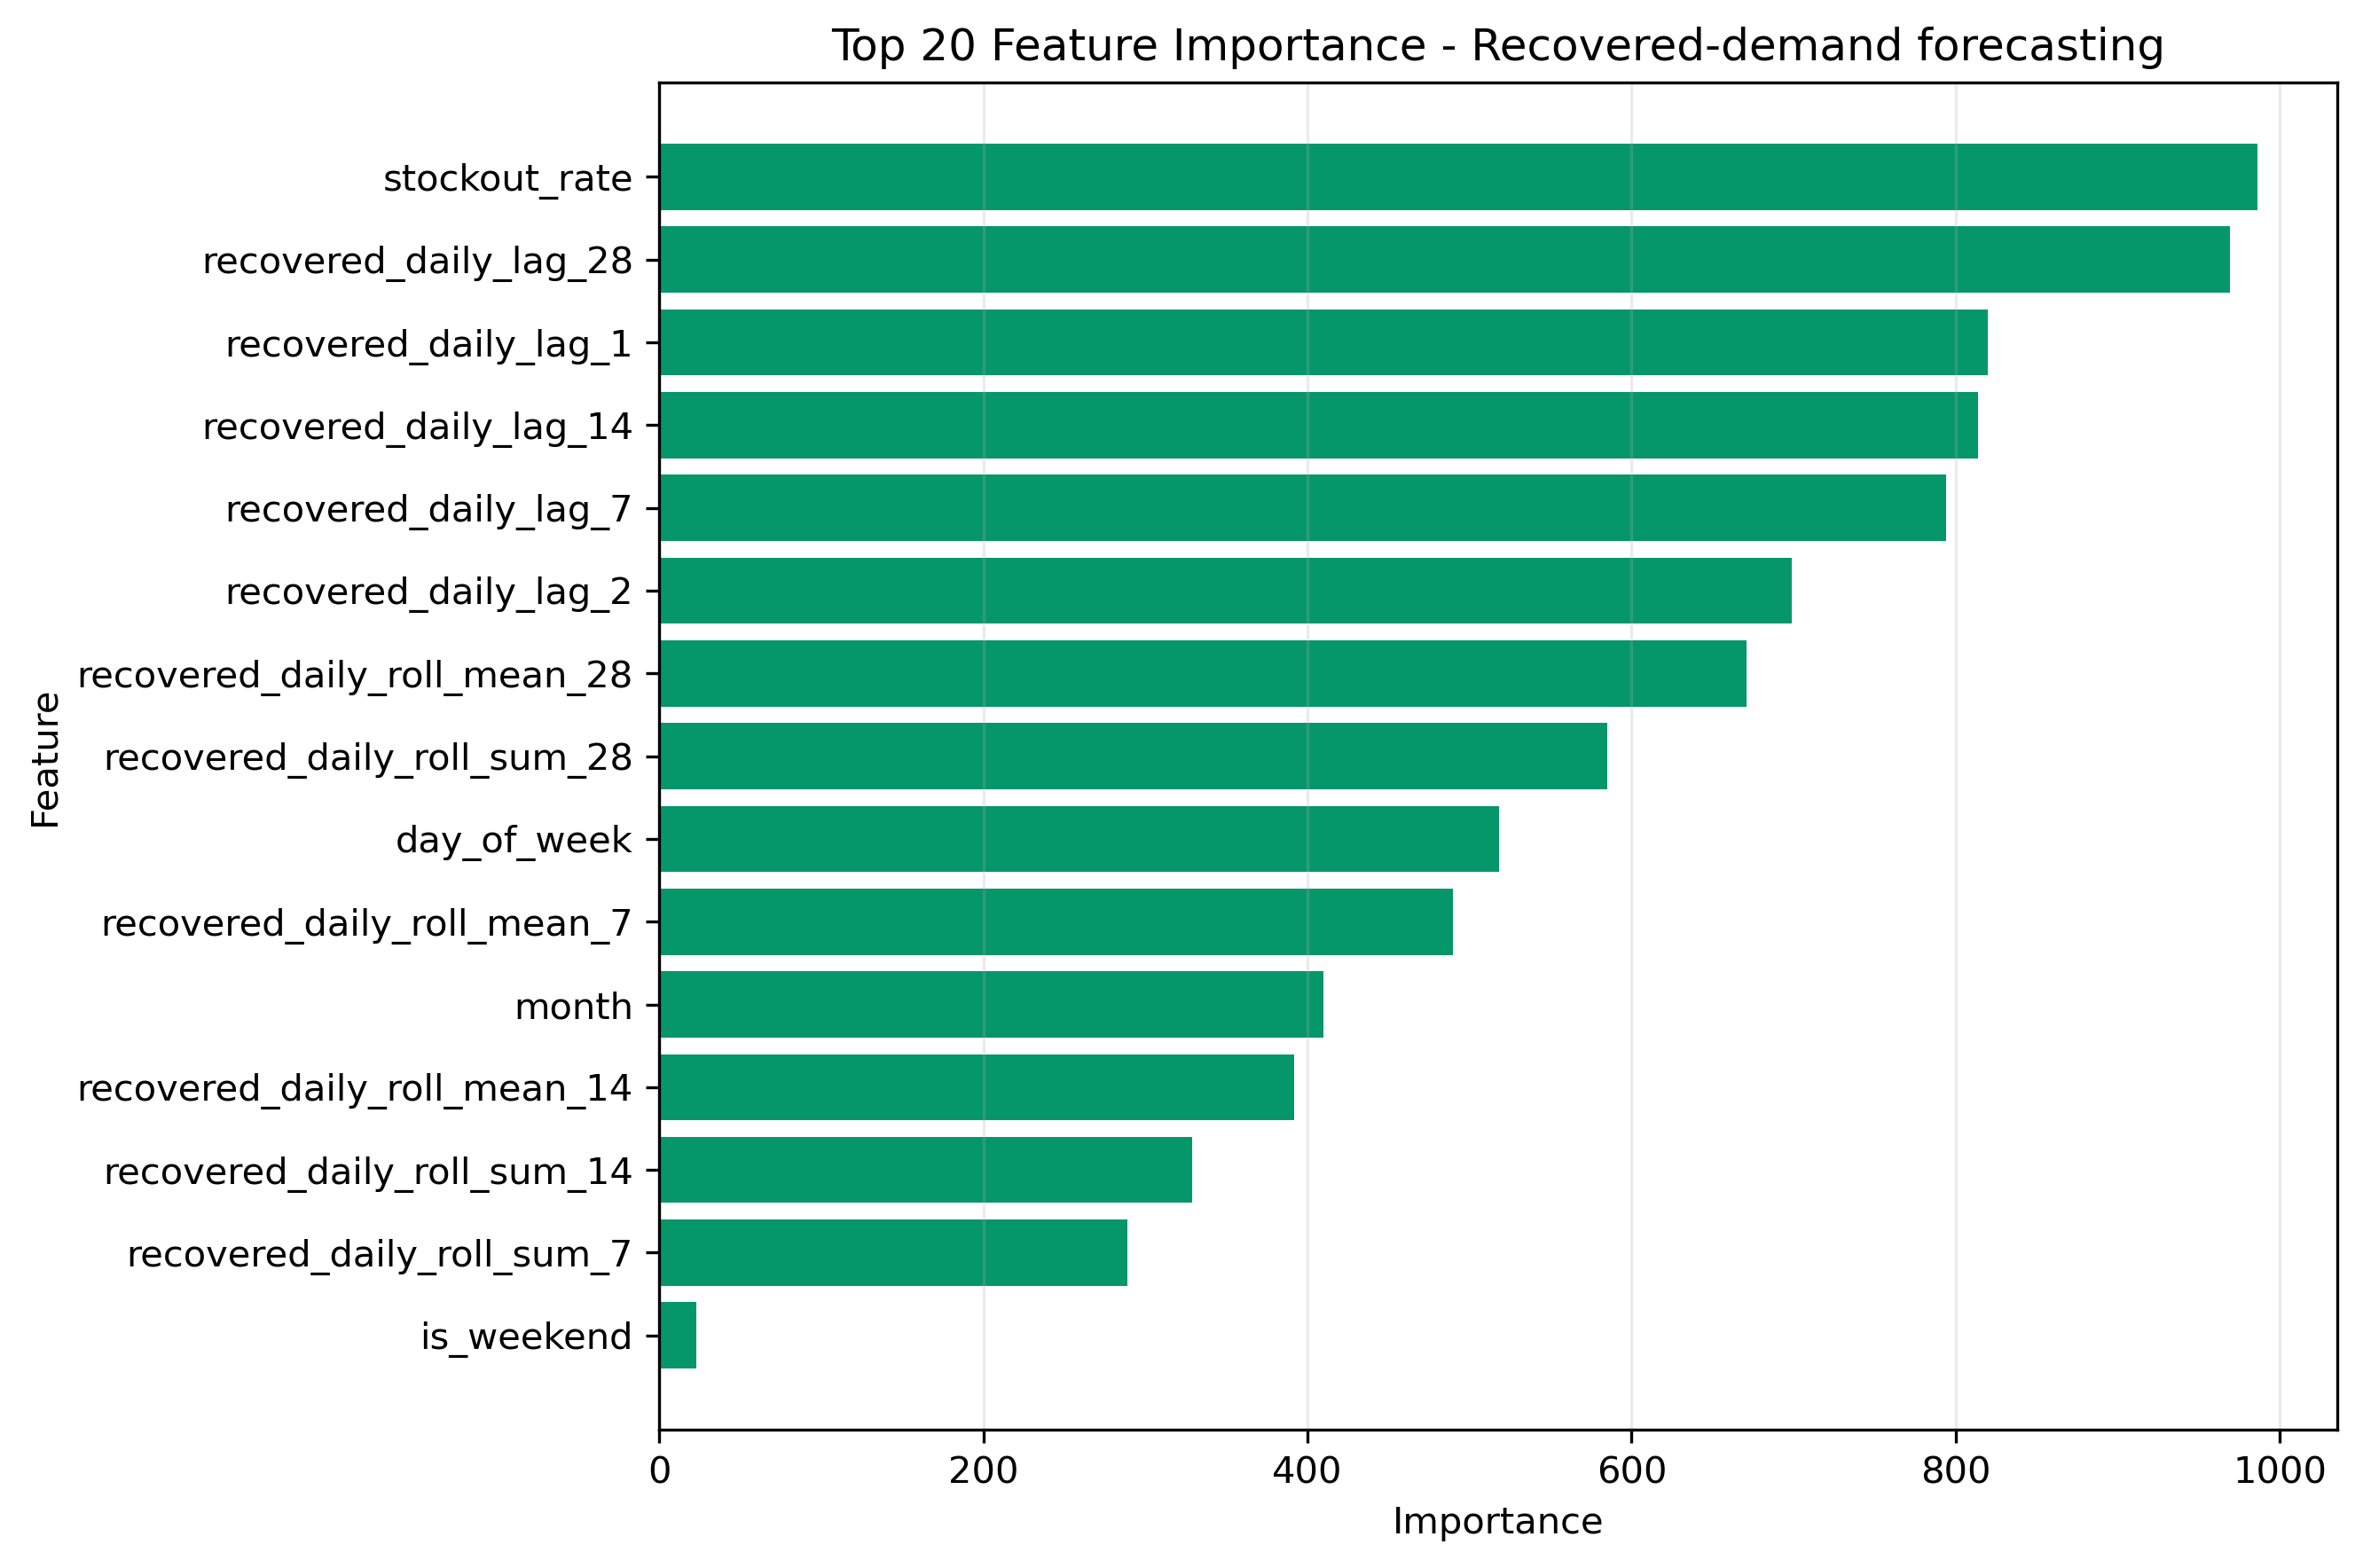
\includegraphics[width=0.78\linewidth]{../figures/owner_recovereddemand_forecasting_feature_importance_top20.png}
    \caption{Top 20 feature importance của mô hình recovered-demand forecasting.}
    \label{fig:vi-owner-feature-importance}
\end{figure}



\section{Phân tích bổ sung trên benchmark observed-sales}
Các phân tích trong mục này được giữ như sanity check cho pipeline feature engineering ban đầu.
Chúng không phải kết quả chính của đồ án, vì target của chúng vẫn là observed sales.
Tuy nhiên, chúng giúp giải thích vì sao các nhóm đặc trưng thời gian, promotion, weather và stockout-aware vẫn hữu ích trước khi chuyển sang mô hình two-stage.

\subsection{Ablation study}
Ablation study kiểm tra giá trị gia tăng của promotion, weather và stockout features trên benchmark LightGBM observed-sales.

\begin{table}[H]
\centering
\caption{Kết quả ablation LightGBM trên observed-sales benchmark}
\resizebox{\linewidth}{!}{%
\begin{tabular}{lllllll}
\toprule
Horizon & Feature set & RMSE & MAE & WAPE & sMAPE & Train rows used \\
\midrule
1 & Lag + Calendar + Promotion + Weather + Stockout & 0.0972 & 0.0525 & 1.0710 & 1.7026 & 500000 \\
1 & Lag + Calendar + Promotion & 0.0983 & 0.0544 & 1.1109 & 1.7125 & 500000 \\
1 & Lag + Calendar + Promotion + Weather & 0.0991 & 0.0546 & 1.1143 & 1.7122 & 500000 \\
1 & Lag + Calendar & 0.0987 & 0.0546 & 1.1153 & 1.7118 & 500000 \\
\bottomrule
\end{tabular}
}
\end{table}


\begin{figure}[H]
    \centering
    
\includegraphics[width=0.92\linewidth]{../figures/ablation_wape_h1.png}
    \caption{Ablation theo WAPE cho h=1.}
    \label{fig:vi-ablation}
\end{figure}


\subsection{Phân tích stockout và nhu cầu bị kiểm duyệt}
Khi hết hàng, doanh số quan sát được có thể thấp hơn nhu cầu thực.
Phân tích lost-sales proxy ban đầu dùng rolling mean 168 giờ để minh họa cơ chế censoring; pipeline chính sau đó thay proxy thô này bằng expanding-window latent demand recovery.

\begin{table}[H]
\centering
\caption{Tóm tắt stockout-censoring và lost-sales proxy}
\begin{tabular}{ll}
\toprule
Metric & Value \\
\midrule
Observed sales & 482,696 \\
Lost sales proxy during stockout & 107,735 \\
Adjusted demand proxy & 590,432 \\
Stockout row rate & 0.2465 \\
Lost sales proxy / observed sales & 0.2232 \\
\bottomrule
\end{tabular}
\end{table}


\begin{figure}[H]
    \centering
    
\includegraphics[width=0.82\linewidth]{../figures/stockout_lost_sales_proxy_by_hour.png}
    \caption{Doanh số quan sát và lost-sales proxy theo giờ.}
    \label{fig:vi-lost-sales}
\end{figure}


\begin{table}[H]
\centering
\caption{Đánh giá riêng stockout và non-stockout periods}
\resizebox{\linewidth}{!}{%
\begin{tabular}{llllllll}
\toprule
Horizon & Model & Segment & RMSE & MAE & WAPE & sMAPE & N \\
\midrule
1 & LightGBM & non\_stockout\_period & 0.1065 & 0.0609 & 0.9779 & 1.6196 & 1293347 \\
1 & LightGBM & overall & 0.0957 & 0.0513 & 1.0483 & 1.7028 & 1680000 \\
1 & LightGBM & stockout\_period & 0.0427 & 0.0192 & 4.3970 & 1.9813 & 386653 \\
1 & Naive & non\_stockout\_period & 0.1513 & 0.0707 & 1.1348 & 0.6882 & 1293347 \\
1 & Naive & overall & 0.1414 & 0.0609 & 1.2441 & 0.5973 & 1680000 \\
1 & Naive & stockout\_period & 0.1014 & 0.0282 & 6.4489 & 0.2934 & 386653 \\
1 & Ridge & non\_stockout\_period & 0.1116 & 0.0616 & 0.9890 & 1.6465 & 1293347 \\
1 & Ridge & overall & 0.1019 & 0.0546 & 1.1141 & 1.7237 & 1680000 \\
1 & Ridge & stockout\_period & 0.0590 & 0.0310 & 7.0744 & 1.9821 & 386653 \\
1 & SeasonalNaive168 & non\_stockout\_period & 0.1410 & 0.0669 & 1.0731 & 0.6649 & 1293347 \\
1 & SeasonalNaive168 & overall & 0.1323 & 0.0588 & 1.2007 & 0.5970 & 1680000 \\
1 & SeasonalNaive168 & stockout\_period & 0.0977 & 0.0319 & 7.2799 & 0.3697 & 386653 \\
1 & SeasonalNaive24 & non\_stockout\_period & 0.1444 & 0.0678 & 1.0881 & 0.6660 & 1293347 \\
1 & SeasonalNaive24 & overall & 0.1367 & 0.0601 & 1.2260 & 0.5991 & 1680000 \\
1 & SeasonalNaive24 & stockout\_period & 0.1073 & 0.0341 & 7.7945 & 0.3754 & 386653 \\
24 & LightGBM & non\_stockout\_period & 0.1069 & 0.0587 & 0.9386 & 1.6422 & 1291783 \\
24 & LightGBM & overall & 0.0986 & 0.0525 & 1.0695 & 1.7195 & 1680000 \\
24 & LightGBM & stockout\_period & 0.0639 & 0.0319 & 7.2645 & 1.9765 & 388217 \\
24 & Naive & non\_stockout\_period & 0.1448 & 0.0682 & 1.0906 & 0.6682 & 1291783 \\
24 & Naive & overall & 0.1350 & 0.0594 & 1.2094 & 0.5943 & 1680000 \\
24 & Naive & stockout\_period & 0.0957 & 0.0301 & 6.8366 & 0.3484 & 388217 \\
24 & Ridge & non\_stockout\_period & 0.1108 & 0.0630 & 1.0068 & 1.6325 & 1291783 \\
24 & Ridge & overall & 0.1025 & 0.0573 & 1.1663 & 1.7113 & 1680000 \\
24 & Ridge & stockout\_period & 0.0682 & 0.0383 & 8.7163 & 1.9736 & 388217 \\
24 & SeasonalNaive168 & non\_stockout\_period & 0.1413 & 0.0670 & 1.0709 & 0.6664 & 1291783 \\
24 & SeasonalNaive168 & overall & 0.1314 & 0.0582 & 1.1837 & 0.5913 & 1680000 \\
24 & SeasonalNaive168 & stockout\_period & 0.0909 & 0.0287 & 6.5264 & 0.3416 & 388217 \\
24 & SeasonalNaive24 & non\_stockout\_period & 0.1448 & 0.0682 & 1.0906 & 0.6682 & 1291783 \\
24 & SeasonalNaive24 & overall & 0.1350 & 0.0594 & 1.2094 & 0.5943 & 1680000 \\
24 & SeasonalNaive24 & stockout\_period & 0.0957 & 0.0301 & 6.8366 & 0.3484 & 388217 \\
\bottomrule
\end{tabular}
}
\end{table}

\subsection{Kiểm tra độ ổn định và mô hình cổ điển}
Rolling-window evaluation cho thấy hiệu năng LightGBM observed-sales tương đối ổn định giữa hai tuần test.
Ngoài ra, SARIMAX trên chuỗi tổng hợp được dùng như đối chứng time-series cổ điển.
Kết quả cho thấy SARIMAX aggregate không tự động thắng seasonal naive 168h, nhấn mạnh sức mạnh của mùa vụ tuần và sự cần thiết của benchmark.

\begin{table}[H]
\centering
\caption{Rolling-window evaluation trên test set}
\resizebox{\linewidth}{!}{%
\begin{tabular}{lllllllll}
\toprule
Horizon & Model & Window start & Window end & RMSE & MAE & WAPE & sMAPE & N \\
\midrule
1 & LightGBM & 2024-06-18 & 2024-06-24 23:00:00 & 0.0956 & 0.0512 & 1.0556 & 1.7063 & 840000 \\
1 & LightGBM & 2024-06-25 & 2024-07-01 23:00:00 & 0.0958 & 0.0515 & 1.0410 & 1.6994 & 840000 \\
1 & SeasonalNaive168 & 2024-06-18 & 2024-06-24 23:00:00 & 0.1300 & 0.0577 & 1.1883 & 0.5922 & 840000 \\
1 & SeasonalNaive168 & 2024-06-25 & 2024-07-01 23:00:00 & 0.1346 & 0.0600 & 1.2129 & 0.6018 & 840000 \\
24 & LightGBM & 2024-06-18 & 2024-06-24 23:00:00 & 0.0987 & 0.0525 & 1.0679 & 1.7224 & 840000 \\
24 & LightGBM & 2024-06-25 & 2024-07-01 23:00:00 & 0.0985 & 0.0526 & 1.0710 & 1.7166 & 840000 \\
24 & SeasonalNaive168 & 2024-06-18 & 2024-06-24 23:00:00 & 0.1298 & 0.0574 & 1.1669 & 0.5877 & 840000 \\
24 & SeasonalNaive168 & 2024-06-25 & 2024-07-01 23:00:00 & 0.1330 & 0.0590 & 1.2006 & 0.5950 & 840000 \\
\bottomrule
\end{tabular}
}
\end{table}

\begin{table}[H]
\centering
\caption{So sánh SARIMAX tổng hợp với seasonal naive}
\begin{tabular}{lllllll}
\toprule
Model & RMSE & MAE & WAPE & sMAPE & AIC & BIC \\
\midrule
AggregateSARIMAX & 70.2814 & 32.7022 & 0.1335 & 0.1244 & 18,261 & 18,289 \\
AggregateSeasonalNaive168 & 36.2745 & 21.7752 & 0.0889 & 0.1006 &  &  \\
\bottomrule
\end{tabular}
\end{table}


\begin{figure}[H]
    \centering
    
\includegraphics[width=0.92\linewidth]{../figures/aggregate_sarimax_forecast.png}
    \caption{Dự báo SARIMAX trên chuỗi tổng hợp observed-sales.}
    \label{fig:vi-sarimax}
\end{figure}


\section{Kết luận và hạn chế}
Đồ án cuối cùng được tiếp cận theo hướng two-stage: trước hết khôi phục latent demand trong các giờ stockout bằng expanding-window recovery, sau đó forecast trên daily recovered demand.
Khi đánh giá trên recovered latent demand proxy, LightGBM train trên recovered demand đạt WAPE 0.2028, tốt hơn mô hình train trên observed sales với WAPE 0.2442.
Seasonal naive 7 ngày là baseline rất mạnh; vì vậy mô hình kết luận cuối dùng hybrid seasonal-ML chọn trọng số trên validation.
Hybrid đạt WAPE 0.1967 và WPE -0.0726, là kết quả tốt nhất trong nhóm mô hình/baseline đã thử.
Điều này cho thấy hướng two-stage có ích, nhưng cũng nhấn mạnh rằng seasonality tuần là thành phần nền không thể bỏ qua.

Hạn chế chính là recovered demand vẫn là proxy được ước lượng từ mô hình, không phải ground truth nhu cầu thật.
Ngoài ra, diagnostics chính trên rolling 7-day target vẫn còn tự tương quan nhẹ vì các target liên tiếp overlap mạnh; kiểm tra non-overlapping không bác bỏ tự tương quan nhưng chỉ có ít điểm aggregate.
Jarque--Bera vẫn bác bỏ phân phối chuẩn.
Điều này phù hợp với bản chất dữ liệu bán lẻ thưa, nhiều zero và có spike do khuyến mãi/tồn kho.
Hướng phát triển tiếp theo là thử các mô hình recovery chuyên biệt hơn như SAITS, TimesNet, DLinear hoặc ImputeFormer, đồng thời kiểm tra sensitivity của warmup length và block size.

\end{document}
